% Options for packages loaded elsewhere
\PassOptionsToPackage{unicode}{hyperref}
\PassOptionsToPackage{hyphens}{url}
%
\documentclass[
]{book}
\usepackage{lmodern}
\usepackage{amsmath}
\usepackage{ifxetex,ifluatex}
\ifnum 0\ifxetex 1\fi\ifluatex 1\fi=0 % if pdftex
  \usepackage[T1]{fontenc}
  \usepackage[utf8]{inputenc}
  \usepackage{textcomp} % provide euro and other symbols
  \usepackage{amssymb}
\else % if luatex or xetex
  \usepackage{unicode-math}
  \defaultfontfeatures{Scale=MatchLowercase}
  \defaultfontfeatures[\rmfamily]{Ligatures=TeX,Scale=1}
\fi
% Use upquote if available, for straight quotes in verbatim environments
\IfFileExists{upquote.sty}{\usepackage{upquote}}{}
\IfFileExists{microtype.sty}{% use microtype if available
  \usepackage[]{microtype}
  \UseMicrotypeSet[protrusion]{basicmath} % disable protrusion for tt fonts
}{}
\makeatletter
\@ifundefined{KOMAClassName}{% if non-KOMA class
  \IfFileExists{parskip.sty}{%
    \usepackage{parskip}
  }{% else
    \setlength{\parindent}{0pt}
    \setlength{\parskip}{6pt plus 2pt minus 1pt}}
}{% if KOMA class
  \KOMAoptions{parskip=half}}
\makeatother
\usepackage{xcolor}
\IfFileExists{xurl.sty}{\usepackage{xurl}}{} % add URL line breaks if available
\IfFileExists{bookmark.sty}{\usepackage{bookmark}}{\usepackage{hyperref}}
\hypersetup{
  pdftitle={Bookdown 패키지를 사용한 한글책 제작의 기초},
  pdfauthor={서울시립대학교 통계학과 이용희},
  hidelinks,
  pdfcreator={LaTeX via pandoc}}
\urlstyle{same} % disable monospaced font for URLs
\usepackage{color}
\usepackage{fancyvrb}
\newcommand{\VerbBar}{|}
\newcommand{\VERB}{\Verb[commandchars=\\\{\}]}
\DefineVerbatimEnvironment{Highlighting}{Verbatim}{commandchars=\\\{\}}
% Add ',fontsize=\small' for more characters per line
\usepackage{framed}
\definecolor{shadecolor}{RGB}{248,248,248}
\newenvironment{Shaded}{\begin{snugshade}}{\end{snugshade}}
\newcommand{\AlertTok}[1]{\textcolor[rgb]{0.94,0.16,0.16}{#1}}
\newcommand{\AnnotationTok}[1]{\textcolor[rgb]{0.56,0.35,0.01}{\textbf{\textit{#1}}}}
\newcommand{\AttributeTok}[1]{\textcolor[rgb]{0.77,0.63,0.00}{#1}}
\newcommand{\BaseNTok}[1]{\textcolor[rgb]{0.00,0.00,0.81}{#1}}
\newcommand{\BuiltInTok}[1]{#1}
\newcommand{\CharTok}[1]{\textcolor[rgb]{0.31,0.60,0.02}{#1}}
\newcommand{\CommentTok}[1]{\textcolor[rgb]{0.56,0.35,0.01}{\textit{#1}}}
\newcommand{\CommentVarTok}[1]{\textcolor[rgb]{0.56,0.35,0.01}{\textbf{\textit{#1}}}}
\newcommand{\ConstantTok}[1]{\textcolor[rgb]{0.00,0.00,0.00}{#1}}
\newcommand{\ControlFlowTok}[1]{\textcolor[rgb]{0.13,0.29,0.53}{\textbf{#1}}}
\newcommand{\DataTypeTok}[1]{\textcolor[rgb]{0.13,0.29,0.53}{#1}}
\newcommand{\DecValTok}[1]{\textcolor[rgb]{0.00,0.00,0.81}{#1}}
\newcommand{\DocumentationTok}[1]{\textcolor[rgb]{0.56,0.35,0.01}{\textbf{\textit{#1}}}}
\newcommand{\ErrorTok}[1]{\textcolor[rgb]{0.64,0.00,0.00}{\textbf{#1}}}
\newcommand{\ExtensionTok}[1]{#1}
\newcommand{\FloatTok}[1]{\textcolor[rgb]{0.00,0.00,0.81}{#1}}
\newcommand{\FunctionTok}[1]{\textcolor[rgb]{0.00,0.00,0.00}{#1}}
\newcommand{\ImportTok}[1]{#1}
\newcommand{\InformationTok}[1]{\textcolor[rgb]{0.56,0.35,0.01}{\textbf{\textit{#1}}}}
\newcommand{\KeywordTok}[1]{\textcolor[rgb]{0.13,0.29,0.53}{\textbf{#1}}}
\newcommand{\NormalTok}[1]{#1}
\newcommand{\OperatorTok}[1]{\textcolor[rgb]{0.81,0.36,0.00}{\textbf{#1}}}
\newcommand{\OtherTok}[1]{\textcolor[rgb]{0.56,0.35,0.01}{#1}}
\newcommand{\PreprocessorTok}[1]{\textcolor[rgb]{0.56,0.35,0.01}{\textit{#1}}}
\newcommand{\RegionMarkerTok}[1]{#1}
\newcommand{\SpecialCharTok}[1]{\textcolor[rgb]{0.00,0.00,0.00}{#1}}
\newcommand{\SpecialStringTok}[1]{\textcolor[rgb]{0.31,0.60,0.02}{#1}}
\newcommand{\StringTok}[1]{\textcolor[rgb]{0.31,0.60,0.02}{#1}}
\newcommand{\VariableTok}[1]{\textcolor[rgb]{0.00,0.00,0.00}{#1}}
\newcommand{\VerbatimStringTok}[1]{\textcolor[rgb]{0.31,0.60,0.02}{#1}}
\newcommand{\WarningTok}[1]{\textcolor[rgb]{0.56,0.35,0.01}{\textbf{\textit{#1}}}}
\usepackage{longtable,booktabs}
\usepackage{calc} % for calculating minipage widths
% Correct order of tables after \paragraph or \subparagraph
\usepackage{etoolbox}
\makeatletter
\patchcmd\longtable{\par}{\if@noskipsec\mbox{}\fi\par}{}{}
\makeatother
% Allow footnotes in longtable head/foot
\IfFileExists{footnotehyper.sty}{\usepackage{footnotehyper}}{\usepackage{footnote}}
\makesavenoteenv{longtable}
\usepackage{graphicx}
\makeatletter
\def\maxwidth{\ifdim\Gin@nat@width>\linewidth\linewidth\else\Gin@nat@width\fi}
\def\maxheight{\ifdim\Gin@nat@height>\textheight\textheight\else\Gin@nat@height\fi}
\makeatother
% Scale images if necessary, so that they will not overflow the page
% margins by default, and it is still possible to overwrite the defaults
% using explicit options in \includegraphics[width, height, ...]{}
\setkeys{Gin}{width=\maxwidth,height=\maxheight,keepaspectratio}
% Set default figure placement to htbp
\makeatletter
\def\fps@figure{htbp}
\makeatother
\setlength{\emergencystretch}{3em} % prevent overfull lines
\providecommand{\tightlist}{%
  \setlength{\itemsep}{0pt}\setlength{\parskip}{0pt}}
\setcounter{secnumdepth}{5}
%----- my options----------------
\usepackage[hangul]{kotex}
\usepackage{bm}
\usepackage{fullpage}

\newcommand{\pardiff}[2]{\frac{\partial #1}{\partial #2 }}
\newcommand{\pardiffl}[2]{{\partial #1}/{\partial #2 }}
\newcommand{\pardiffd}[2]{\frac{\partial^2 #1}{\partial #2^t \partial #2 }}
\newcommand{\pardiffdd}[3]{\frac{\partial^2 #1}{\partial #2 \partial #3 }}

\usepackage{hyperref}
\hypersetup{
    colorlinks=true,
    linkcolor=blue,
    filecolor=blue,      
    urlcolor=blue,
}

\urlstyle{same}


%--------- from bookdown.org --------------

\usepackage{booktabs}



\usepackage{framed,color}
\definecolor{shadecolor}{RGB}{248,248,248}

\renewcommand{\textfraction}{0.05}
\renewcommand{\topfraction}{0.8}
\renewcommand{\bottomfraction}{0.8}
\renewcommand{\floatpagefraction}{0.75}

%\renewenvironment{quote}{\begin{VF}}{\end{VF}}
%\let\oldhref\href
%\renewcommand{\href}[2]{#2\footnote{\url{#1}}}

\makeatletter
\newenvironment{kframe}{%
\medskip{}
\setlength{\fboxsep}{.8em}
 \def\at@end@of@kframe{}%
 \ifinner\ifhmode%
  \def\at@end@of@kframe{\end{minipage}}%
  \begin{minipage}{\columnwidth}%
 \fi\fi%
 \def\FrameCommand##1{\hskip\@totalleftmargin \hskip-\fboxsep
 \colorbox{shadecolor}{##1}\hskip-\fboxsep
     % There is no \\@totalrightmargin, so:
     \hskip-\linewidth \hskip-\@totalleftmargin \hskip\columnwidth}%
 \MakeFramed {\advance\hsize-\width
   \@totalleftmargin\z@ \linewidth\hsize
   \@setminipage}}%
 {\par\unskip\endMakeFramed%
 \at@end@of@kframe}
\makeatother

\makeatletter

\@ifundefined{Shaded}{
}{\renewenvironment{Shaded}{\begin{kframe}}{\end{kframe}}}
\makeatother

\newenvironment{rmdblock}[1]
  {
  \begin{itemize}
  \renewcommand{\labelitemi}{
    \raisebox{-.7\height}[0pt][0pt]{
      {\setkeys{Gin}{width=3em,keepaspectratio}\includegraphics{images/#1}}
    }
  }
  \setlength{\fboxsep}{1em}
  \begin{kframe}
  \item
  }
  {
  \end{kframe}
  \end{itemize}
  }
  
\newenvironment{rmdnote}
  {\begin{rmdblock}{note}}
  {\end{rmdblock}}
  
\newenvironment{rmdcaution}
  {\begin{rmdblock}{caution}}
  {\end{rmdblock}}
  
\newenvironment{rmdimportant}
  {\begin{rmdblock}{important}}
  {\end{rmdblock}}
  
\newenvironment{rmdtip}
  {\begin{rmdblock}{tip}}
  {\end{rmdblock}}
  
\newenvironment{rmdwarning}
  {\begin{rmdblock}{warning}}
  {\end{rmdblock}}
  


\usepackage{makeidx}
\makeindex

\urlstyle{tt}

\usepackage{amsthm}
\makeatletter
 \def\thm@space@setup{%
   \thm@preskip=8pt plus 2pt minus 4pt
   \thm@postskip=\thm@preskip
}
\makeatother

\frontmatter
\usepackage{booktabs}
\usepackage{longtable}
\usepackage{array}
\usepackage{multirow}
\usepackage{wrapfig}
\usepackage{float}
\usepackage{colortbl}
\usepackage{pdflscape}
\usepackage{tabu}
\usepackage{threeparttable}
\usepackage{threeparttablex}
\usepackage[normalem]{ulem}
\usepackage{makecell}
\usepackage{xcolor}
\usepackage{multicol}
\usepackage{hhline}
\usepackage{hyperref}
\ifluatex
  \usepackage{selnolig}  % disable illegal ligatures
\fi
\usepackage[]{natbib}
\bibliographystyle{apalike}

\title{Bookdown 패키지를 사용한 한글책 제작의 기초}
\author{서울시립대학교 통계학과 이용희}
\date{2021-05-16}

\usepackage{amsthm}
\newtheorem{theorem}{Theorem}[chapter]
\newtheorem{lemma}{Lemma}[chapter]
\newtheorem{corollary}{Corollary}[chapter]
\newtheorem{proposition}{Proposition}[chapter]
\newtheorem{conjecture}{Conjecture}[chapter]
\theoremstyle{definition}
\newtheorem{definition}{정의}[chapter]
\theoremstyle{definition}
\newtheorem{example}{예제}[chapter]
\theoremstyle{definition}
\newtheorem{exercise}{Exercise}[chapter]
\theoremstyle{definition}
\newtheorem{hypothesis}{Hypothesis}[chapter]
\theoremstyle{remark}
\newtheorem*{remark}{참고}
\newtheorem*{solution}{Solution}
\begin{document}
\maketitle

{
\setcounter{tocdepth}{1}
\tableofcontents
}
\hypertarget{uxac1cuxc694}{%
\chapter*{개요}\label{uxac1cuxc694}}


이 책은 \texttt{bookdown} 패키지를 이용하여 \textbf{한글로 수식, 그림, 표를 포함한 책을 작성할 때} 필요한 사항과 유용한 팁을 수록한 안내서입니다.

\texttt{bookdown} 패키지의 기초와 자세한 사용법은 \href{https://bookdown.org/yihui/bookdown/}{bookdown package documentation} 와 \href{https://rmarkdown.rstudio.com/}{Rmarkdown documentation} 을 참조하세오.

\texttt{bookdown} 패키지를 이용하여 책을 만들려면 먼저 다음과 같이 패키지를 설치해야 합니다.

\begin{Shaded}
\begin{Highlighting}[]
\FunctionTok{install.packages}\NormalTok{(}\StringTok{"bookdown"}\NormalTok{)}
\CommentTok{\# or the development version}
\CommentTok{\# devtools::install\_github("rstudio/bookdown")}
\end{Highlighting}
\end{Shaded}

그리고 이 책에서 이용한 패키지의 목록은 다음과 같습니다.

\begin{verbatim}
library(dplyr)
library(tidyr)
library(ggplot2)
library(kableExtra)
library(equatiomatic)
library(sjPlot)
library(sjmisc)
library(sjlabelled)
library(modelsummary)
library(flextable)
library(lme4)
library(xfun)
\end{verbatim}

\begin{Shaded}
\begin{Highlighting}[]
\CommentTok{\# automatically create a bib database for R packages}
\NormalTok{knitr}\SpecialCharTok{::}\FunctionTok{write\_bib}\NormalTok{(}\FunctionTok{c}\NormalTok{(}
  \FunctionTok{.packages}\NormalTok{(), }\StringTok{\textquotesingle{}bookdown\textquotesingle{}}\NormalTok{, }\StringTok{\textquotesingle{}knitr\textquotesingle{}}\NormalTok{, }\StringTok{\textquotesingle{}rmarkdown\textquotesingle{}}
\NormalTok{), }\StringTok{\textquotesingle{}packages.bib\textquotesingle{}}\NormalTok{)}
\end{Highlighting}
\end{Shaded}

\mainmatter

\hypertarget{intro}{%
\chapter{책의 구성요소와 형식}\label{intro}}

\hypertarget{uxcc45-uxad6cuxc131uxc694uxc18cuxc758-uxc9c0uxc815uxacfc-uxcc38uxc870}{%
\section{책 구성요소의 지정과 참조}\label{uxcc45-uxad6cuxc131uxc694uxc18cuxc758-uxc9c0uxc815uxacfc-uxcc38uxc870}}

\texttt{Bookdown} 에서는 하나의 \texttt{Rmd} 화일이 하나의 장(chapter)이 된다. 따라서 하나의 장에 대한 \texttt{Rmd} 화일은 처음에 다음과 같이 \texttt{\#} 으로 장의 이름을 지정한다. 다음으로 하위 절 등의 제목은\texttt{\#\#}, \texttt{\#\#\#} 순으로 지정한다.

장 이름을 참조하는 장 이름을 정의하는 문장 뒤에 \texttt{\{\#label\}} 을 붙여준다. 장을 참조하는 방법은 명령문 \texttt{\textbackslash{}@ref(label)} 으로 참조한다. (예: 다음 내용은 \ref{intro} 장에 나타나 있다).

\begin{Shaded}
\begin{Highlighting}[]
\FunctionTok{\# 소개 \{\#intro\}}

\FunctionTok{\#\#  공식}

\FunctionTok{\#\#\# 설명}
\end{Highlighting}
\end{Shaded}

\begin{rmdcaution}
장의 이름이 한글인 경우 참조문 \texttt{\{\#label\}}을 붙여주지 않으면 오류가 나오는 경우가 있으니 꼭 붙여주자.
\end{rmdcaution}

\hypertarget{uxad6cuxc131uxc694uxc18cuxc758-uxad6cuxc870}{%
\section{구성요소의 구조}\label{uxad6cuxc131uxc694uxc18cuxc758-uxad6cuxc870}}

책의 구성요소는 다음과 같이 \texttt{part}, \texttt{chapter}, \texttt{appendix} 등으로 구분된다. \texttt{\{-\}} 를 뒤에 붙이면 장이나 절의 번호가 붙지 않는다.

\begin{Shaded}
\begin{Highlighting}[]
\FunctionTok{\# (PART) Part I \{{-}\} }

\FunctionTok{\# Prefeace \{{-}\}}

\FunctionTok{\# Chapter One}

\FunctionTok{\# Chapter Two}

\FunctionTok{\# (PART) Part II \{{-}\} }

\FunctionTok{\# Chapter Three}

\FunctionTok{\# (APPENDIX) Appendix \{{-}\} }

\FunctionTok{\# Appendix A}

\FunctionTok{\# Appendix B}
\end{Highlighting}
\end{Shaded}

\hypertarget{uxad6cuxc131uxc694uxc18c-uxc774uxb984uxc758-uxbcc0uxacbd}{%
\section{구성요소 이름의 변경}\label{uxad6cuxc131uxc694uxc18c-uxc774uxb984uxc758-uxbcc0uxacbd}}

책에서 나오는 chapter, section 과 equation, figure 등의 제목을 영문에서 한글로 바꾸려면
\texttt{\_bookdown.yml} 에 댜음과 같은 명령어를 추가합니다.

\begin{Shaded}
\begin{Highlighting}[]
\AnnotationTok{language:}
\NormalTok{  label:}
\NormalTok{    fig: "그림 "}
\NormalTok{    tab: "표 "}
\NormalTok{    eq:  "공식 "}
\NormalTok{    def: \textquotesingle{}정의 \textquotesingle{}}
\NormalTok{    exm: \textquotesingle{}예제 \textquotesingle{}}
\NormalTok{    proof: \textquotesingle{}증명. \textquotesingle{}}
\NormalTok{    remark: \textquotesingle{}참고. \textquotesingle{}}
\NormalTok{  ui:}
\NormalTok{    chapter\_name: }\CommentTok{[}\OtherTok{"제 ", " 장"}\CommentTok{]}
\NormalTok{    appendix\_name: }\CommentTok{[}\OtherTok{"부록 ", ": "}\CommentTok{]}
\end{Highlighting}
\end{Shaded}

\hypertarget{uxbe14uxb7ed-uxc694uxc18c}{%
\section{블럭 요소}\label{uxbe14uxb7ed-uxc694uxc18c}}

중요한 내용이나 강조하고 싶은 내용을 블럭으로 만들 때 다음과 같은 블럭 명령어 \texttt{block2} 를 사용한다.

\begin{rmdcaution}
블럭 요소 안에서는 markdown 의 item 를 구성하는 형식들(\texttt{-}, \texttt{+}, \texttt{*}) 등이 나타나면 PDF 로 책을 만들때 오류가 자주 나타나므로 이용하지 않는 것이 좋다.
\end{rmdcaution}

\begin{Shaded}
\begin{Highlighting}[]
\InformationTok{\textasciigrave{}\textasciigrave{}\textasciigrave{}\{block2, type=\textquotesingle{}rmdnote\textquotesingle{}, eval=F\}}
\InformationTok{이 책에서 사용된 기호, 표기법, 프로그램의 규칙과 쓰임은 다음과 같습니다.}

\InformationTok{스칼라(scalar)와 일변량 확률변수는 일반적으로  보통 글씨체의 소문자로  표기한다. 특별한 이유가     있는 경우 대문자로 표시할 것이다. }
\InformationTok{벡터, 행렬, 다변량 확률벡터는 굵은 글씨체로 표기한다.}
\InformationTok{\textasciigrave{}\textasciigrave{}\textasciigrave{}}
\end{Highlighting}
\end{Shaded}

\begin{rmdnote}
이 책에서 사용된 기호, 표기법, 프로그램의 규칙과 쓰임은 다음과 같습니다.

스칼라(scalar)와 일변량 확률변수는 일반적으로 보통 글씨체의 소문자로 표기한다. 특별한 이유가 있는 경우 대문자로 표시할 것이다.

벡터, 행렬, 다변량 확률벡터는 굵은 글씨체로 표기한다.
\end{rmdnote}

\texttt{bookdown} 패키지에서 제공하는 블럭의 종류(\texttt{type})는 다음과 같다.

\begin{itemize}
\item
  \texttt{rmdimportant}
\item
  \texttt{rmdcaution}
\item
  \texttt{rmdnote}
\item
  \texttt{rmdcaution}
\item
  \texttt{rmdwarning}
\end{itemize}

\hypertarget{uxcc38uxace0uxbb38uxd5cc}{%
\section{참고문헌}\label{uxcc38uxace0uxbb38uxd5cc}}

\hypertarget{yml-uxc9c0uxc815}{%
\subsection{YML 지정}\label{yml-uxc9c0uxc815}}

참고 문헌은 지정된 \texttt{bib} 화일에 \texttt{bibtex} 형식으로 넣어준다. \texttt{index.Rmd} 의 yml 형식에 댜음과 같이
\texttt{bib} 화일과 참조 형식을 지정해준다.

\begin{Shaded}
\begin{Highlighting}[]
\AnnotationTok{bibliography:}\CommentTok{ [book.bib, packages.bib]}
\AnnotationTok{biblio{-}style:}\CommentTok{ apalike}
\AnnotationTok{link{-}citations:}\CommentTok{ true}
\end{Highlighting}
\end{Shaded}

\texttt{\_output.yml} 화일에는 PDF 로 출력하는 경우 사용되는 패키지 형식을 다음과 같이 지정한다.

\begin{Shaded}
\begin{Highlighting}[]
\NormalTok{bookdown::pdf\_book:}
\NormalTok{  citation\_package: natbib}
\end{Highlighting}
\end{Shaded}

\hypertarget{bib-uxd654uxc77c}{%
\subsection{BIB 화일}\label{bib-uxd654uxc77c}}

\texttt{packages.bib}는 책에서 사용된 패키지의 참조 화일을 다음과 같은 명령문(\texttt{index.Rmd} 에 포함되어 있다)으로 자동적으로 생성한다.

\begin{Shaded}
\begin{Highlighting}[]
\FunctionTok{\# automatically create a bib database for R packages}
\NormalTok{knitr::write\_bib(c(}
\NormalTok{  .packages(), \textquotesingle{}bookdown\textquotesingle{}, \textquotesingle{}knitr\textquotesingle{}, \textquotesingle{}rmarkdown\textquotesingle{}}
\NormalTok{), \textquotesingle{}packages.bib\textquotesingle{})}
\end{Highlighting}
\end{Shaded}

\texttt{book.bib} 화일에 본분에서 참조할 책이나 논문을 \texttt{bibtex} 형식으로 추가햐면 된다.

\hypertarget{uxcc38uxc870-uxbc29uxbc95}{%
\subsection{참조 방법}\label{uxcc38uxc870-uxbc29uxbc95}}

참조 방법은 \texttt{@key} 또는 \texttt{{[}@key{]}} 를 사용하여 \texttt{{[}{]}} 는 참조가 \texttt{()} 안에 출력된다.

예를 들면 교과서 \citet{xie2015} 는 \texttt{bookdown} 에 대한 매뉴얼이며 다음의 모형은 \citet{battese1988error} 이 제안하였다 \citep{royall1970finite}

\hypertarget{pdf-uxd654uxc77c}{%
\section{PDF 화일}\label{pdf-uxd654uxc77c}}

다음에 나오는 절차들은 Latex 으로 책을 PDF 화일로 만들기 위하여 필요한 작업들이다.

\hypertarget{mainmatter}{%
\subsection{\texorpdfstring{\texttt{\textbackslash{}mainmatter}}{\textbackslash mainmatter}}\label{mainmatter}}

가장 처음으로 나타나는 장의 \texttt{Rmd} 화일의 첫 문장을 \texttt{\textbackslash{}mainmatter} 로 시작한다.

\begin{Shaded}
\begin{Highlighting}[]
\NormalTok{\textbackslash{}mainmatter}

\FunctionTok{\# 책의 구성요소와 형식 \{\#intro\}}
\end{Highlighting}
\end{Shaded}

\hypertarget{backmatter}{%
\subsection{\texorpdfstring{\texttt{\textbackslash{}backmatter}}{\textbackslash backmatter}}\label{backmatter}}

책의 마지막 부분, 즉 부록과 참고문헌 사이에 다음과 같아 써준다.

\begin{Shaded}
\begin{Highlighting}[]
\NormalTok{\textbackslash{}backmatter}

\FunctionTok{\# References \{{-}\}}
\end{Highlighting}
\end{Shaded}

\hypertarget{uxcc38uxc870-uxd615uxc2dduxc758-uxbcc0uxacbd}{%
\subsection{참조 형식의 변경}\label{uxcc38uxc870-uxd615uxc2dduxc758-uxbcc0uxacbd}}

이 책에서는 참조의 형식을 \texttt{\textbackslash{}usepackage\{hyperref\}} 를 이용하여 작성하였다.

만약 참조의 형식을 footnote 형식으로 바꾸려면 \texttt{preample.tex} 에 대름과 같은 명령어를 추가한다.

\begin{Shaded}
\begin{Highlighting}[]
\NormalTok{\textbackslash{}renewenvironment\{quote\}\{\textbackslash{}begin\{VF\}\}\{\textbackslash{}end\{VF\}\}}
\NormalTok{\textbackslash{}let\textbackslash{}oldhref\textbackslash{}href}
\NormalTok{\textbackslash{}renewcommand\{\textbackslash{}href\}}\CommentTok{[}\OtherTok{2}\CommentTok{]}\NormalTok{\{\#2\textbackslash{}footnote\{\textbackslash{}url\{\#1\}\}\}}
\end{Highlighting}
\end{Shaded}

\hypertarget{math}{%
\chapter{수식}\label{math}}

\hypertarget{uxc218uxd559-uxc218uxc2dd}{%
\section{수학 수식}\label{uxc218uxd559-uxc218uxc2dd}}

\hypertarget{uxc218uxc2dd-uxc0acuxc6a9-uxd658uxacbd-uxb9ccuxb4e4uxae30}{%
\subsection{수식 사용 환경 만들기}\label{uxc218uxc2dd-uxc0acuxc6a9-uxd658uxacbd-uxb9ccuxb4e4uxae30}}

Latex 으로 수식을 사용하는 경우 \texttt{\_outout.yml} 화일에 필요한 새로운 명령이나 패키지를 다음과 같이 별도의 화일로 지정할 수 있다.

\begin{itemize}
\tightlist
\item
  HTML with gitbook
\end{itemize}

\begin{verbatim}
bookdown::gitbook:
  includes:
    before_body: preamble-mathjax.tex
\end{verbatim}

\begin{itemize}
\tightlist
\item
  PDF with Latex
\end{itemize}

\begin{verbatim}
bookdown::pdf_book:
  includes:
    in_header: latex/preamble.tex
    before_body: latex/before_body.tex
    after_body: latex/after_body.tex
\end{verbatim}

위에서 언급한 PDF 화일을 위한 Latex 화일들은 \href{https://github.com/rstudio/bookdown/tree/master/inst/examples/latex}{여기서} 찾을 수 있다.

\texttt{gitbook} 형식을 이용하여 HTML 로 책을 만드는 경우 MathJax 에 포함되지 않은 Latex 패키지는 사용할 수 없다. 예를 들어 문자를 굵은 글씨체로 만들어 주는 Latex 패키지 \texttt{bm} 을 사용하지 못한다. 따라서 이러한 경우는 다음과 같이 새로운 명령어를 만들어서 \texttt{preamble-mathjax.tex} 에 넣어준다. MathJax 의 명령문을 정의하는 경우는 \texttt{\textbackslash{}(} 과 \texttt{\textbackslash{})} 사이에 넣어 주어야 한다.

\begin{itemize}
\tightlist
\item
  \texttt{preamble-mathjax.tex} 의 내용
\end{itemize}

\begin{Shaded}
\begin{Highlighting}[]
\SpecialStringTok{\textbackslash{}(}
\SpecialCharTok{\textbackslash{}newcommand}\SpecialStringTok{\{}\SpecialCharTok{\textbackslash{}bm}\SpecialStringTok{\}[1]\{}\SpecialCharTok{\textbackslash{}boldsymbol}\SpecialStringTok{\{}\SpecialCharTok{\textbackslash{}mathbf}\SpecialStringTok{\{\#1\}\}\}}
\SpecialCharTok{\textbackslash{}newcommand}\SpecialStringTok{\{}\SpecialCharTok{\textbackslash{}pardiff}\SpecialStringTok{\}[2]\{}\SpecialCharTok{\textbackslash{}frac}\SpecialStringTok{\{}\SpecialCharTok{\textbackslash{}partial}\SpecialStringTok{ \#1\}\{}\SpecialCharTok{\textbackslash{}partial}\SpecialStringTok{ \#2 \}\}}
\SpecialCharTok{\textbackslash{}newcommand}\SpecialStringTok{\{}\SpecialCharTok{\textbackslash{}pardiffl}\SpecialStringTok{\}[2]\{\{}\SpecialCharTok{\textbackslash{}partial}\SpecialStringTok{ \#1\}/\{}\SpecialCharTok{\textbackslash{}partial}\SpecialStringTok{ \#2 \}\}}
\SpecialCharTok{\textbackslash{}newcommand}\SpecialStringTok{\{}\SpecialCharTok{\textbackslash{}pardiffd}\SpecialStringTok{\}[2]\{}\SpecialCharTok{\textbackslash{}frac}\SpecialStringTok{\{}\SpecialCharTok{\textbackslash{}partial}\SpecialStringTok{\^{}2 \#1\}\{}\SpecialCharTok{\textbackslash{}partial}\SpecialStringTok{ \#2\^{}t }\SpecialCharTok{\textbackslash{}partial}\SpecialStringTok{ \#2 \}\}}
\SpecialCharTok{\textbackslash{}newcommand}\SpecialStringTok{\{}\SpecialCharTok{\textbackslash{}pardiffdd}\SpecialStringTok{\}[3]\{}\SpecialCharTok{\textbackslash{}frac}\SpecialStringTok{\{}\SpecialCharTok{\textbackslash{}partial}\SpecialStringTok{\^{}2 \#1\}\{}\SpecialCharTok{\textbackslash{}partial}\SpecialStringTok{ \#2 }\SpecialCharTok{\textbackslash{}partial}\SpecialStringTok{ \#3 \}\}}
\SpecialStringTok{\textbackslash{})}
\end{Highlighting}
\end{Shaded}

\hypertarget{uxc218uxc2dd-uxcc38uxc870}{%
\subsection{수식 참조}\label{uxc218uxc2dd-uxcc38uxc870}}

수식에 번호를 붙이고 라벨을 지정하여 참조하려면 다음과 같은 명령어를 사용한다. 라벨은 \texttt{(\textbackslash{}\#eq:label)} 의 형식으로 지정한다. \textbf{주의할 점은 수식의 라벨은 반드시 \texttt{eq:} 으로 시작되어야 한다.} \texttt{Bookdown} 패키지에서는 수식, 표, 그림 등의 라벨을 만들 경우 꼭 앞에 붙여주어야 하는 접두어(prefix)가 있으니 주의해야 한다.

\begin{Shaded}
\begin{Highlighting}[]
\KeywordTok{\textbackslash{}begin}\NormalTok{\{}\ExtensionTok{equation}\NormalTok{\}}\SpecialStringTok{ }
\SpecialStringTok{  y\_\{i\}= }\SpecialCharTok{\textbackslash{}beta}\SpecialStringTok{\_0 + }\SpecialCharTok{\textbackslash{}beta}\SpecialStringTok{\_1 x\_\{i\} + e\_\{i\}}
\SpecialStringTok{  (}\SpecialCharTok{\textbackslash{}\#}\SpecialStringTok{eq:reg)}
\KeywordTok{\textbackslash{}end}\NormalTok{\{}\ExtensionTok{equation}\NormalTok{\} }
\end{Highlighting}
\end{Shaded}

위의 명령어는 다음과 같이 출력된다.

\begin{equation} 
  y_{i}= \beta_0 + \beta_1 x_{i} + e_{i}
\label{eq:reg}
\end{equation}

위의 수식을 참조하려면 명령문 \texttt{\textbackslash{}@ref(eq:reg)} 으로 참조한다. 예를 들면 식 \eqref{eq:reg} 을 참조하세요.

\hypertarget{uxd328uxd0a4uxc9c0-equatiomatic}{%
\section{\texorpdfstring{패키지 \texttt{equatiomatic}}{패키지 equatiomatic}}\label{uxd328uxd0a4uxc9c0-equatiomatic}}

패키지 \texttt{equatiomatic} 를 이용하면 \texttt{R} 에서 얻은 결과를 이용하여 모형 추정식이나 추정식의 결과를
쉽게 나타낼 수 있다. 이제 몇 개의 예제를 살펴보자. 패키지 \texttt{equatiomatic} 에서 수식을 출력하는
자세한 방법은 \href{https://datalorax.github.io/equatiomatic/index.html}{패키지 설명서} 를 참조하자.

이제 위에서 본 \texttt{cars} 자료를 가지고 선형회귀모형 \eqref{eq:reg} 에 나타난 회귀계수를 추정해보자. 아래는 \texttt{R} 프로그램에서 함수 \texttt{lm}을 이용한 추정결과이다.

\begin{Shaded}
\begin{Highlighting}[]
\NormalTok{lmOut }\OtherTok{\textless{}{-}} \FunctionTok{lm}\NormalTok{(dist}\SpecialCharTok{\textasciitilde{}}\NormalTok{speed, }\AttributeTok{data=}\NormalTok{cars)}
\FunctionTok{summary}\NormalTok{(lmOut)}
\end{Highlighting}
\end{Shaded}

\begin{verbatim}
## 
## Call:
## lm(formula = dist ~ speed, data = cars)
## 
## Residuals:
##     Min      1Q  Median      3Q     Max 
## -29.069  -9.525  -2.272   9.215  43.201 
## 
## Coefficients:
##             Estimate Std. Error t value Pr(>|t|)    
## (Intercept) -17.5791     6.7584  -2.601   0.0123 *  
## speed         3.9324     0.4155   9.464 1.49e-12 ***
## ---
## Signif. codes:  0 '***' 0.001 '**' 0.01 '*' 0.05 '.' 0.1 ' ' 1
## 
## Residual standard error: 15.38 on 48 degrees of freedom
## Multiple R-squared:  0.6511, Adjusted R-squared:  0.6438 
## F-statistic: 89.57 on 1 and 48 DF,  p-value: 1.49e-12
\end{verbatim}

위에서 주어진 선형회귀모형 \eqref{eq:reg}은 다음과 같은 회귀식을 추정한다.

\begin{Shaded}
\begin{Highlighting}[]
\NormalTok{equatiomatic}\SpecialCharTok{::}\FunctionTok{extract\_eq}\NormalTok{(lmOut, }\AttributeTok{intercept =} \StringTok{"beta"}\NormalTok{,  }\AttributeTok{use\_coefs =} \ConstantTok{FALSE}\NormalTok{)}
\end{Highlighting}
\end{Shaded}

\[
\operatorname{dist} = \beta_{0} + \beta_{1}(\operatorname{speed}) + \epsilon
\]

추정 결과를 이용하면 자동차의 속도(\(x\) = \texttt{speed})와 제동거리(\(y\) = \texttt{dist})의 관계는 다음과 같은 회귀식으로 나타낼 수 있다.

\begin{Shaded}
\begin{Highlighting}[]
\NormalTok{equatiomatic}\SpecialCharTok{::}\FunctionTok{extract\_eq}\NormalTok{(lmOut, }\AttributeTok{intercept =} \StringTok{"beta"}\NormalTok{, }\AttributeTok{use\_coefs =} \ConstantTok{TRUE}\NormalTok{)}
\end{Highlighting}
\end{Shaded}

\[
\operatorname{\widehat{dist}} = -17.58 + 3.93(\operatorname{speed})
\]

다음은 패키지 \texttt{lme4}의 \texttt{sleepstudy}를 선형혼합모형으로 적합한 결과를 보여준다.

\begin{Shaded}
\begin{Highlighting}[]
\NormalTok{fm1 }\OtherTok{\textless{}{-}} \FunctionTok{lmer}\NormalTok{(Reaction }\SpecialCharTok{\textasciitilde{}}\NormalTok{ Days }\SpecialCharTok{+}\NormalTok{ (Days}\SpecialCharTok{|}\NormalTok{Subject), sleepstudy)}
\FunctionTok{summary}\NormalTok{(fm1)}
\end{Highlighting}
\end{Shaded}

\begin{verbatim}
## Linear mixed model fit by REML ['lmerMod']
## Formula: Reaction ~ Days + (Days | Subject)
##    Data: sleepstudy
## 
## REML criterion at convergence: 1743.6
## 
## Scaled residuals: 
##     Min      1Q  Median      3Q     Max 
## -3.9536 -0.4634  0.0231  0.4634  5.1793 
## 
## Random effects:
##  Groups   Name        Variance Std.Dev. Corr
##  Subject  (Intercept) 612.10   24.741       
##           Days         35.07    5.922   0.07
##  Residual             654.94   25.592       
## Number of obs: 180, groups:  Subject, 18
## 
## Fixed effects:
##             Estimate Std. Error t value
## (Intercept)  251.405      6.825  36.838
## Days          10.467      1.546   6.771
## 
## Correlation of Fixed Effects:
##      (Intr)
## Days -0.138
\end{verbatim}

\begin{Shaded}
\begin{Highlighting}[]
\NormalTok{equatiomatic}\SpecialCharTok{::}\FunctionTok{extract\_eq}\NormalTok{(fm1, }\AttributeTok{intercept =} \StringTok{"beta"}\NormalTok{, }\AttributeTok{use\_coefs =} \ConstantTok{FALSE}\NormalTok{)}
\end{Highlighting}
\end{Shaded}

\[
\begin{aligned}
  \operatorname{Reaction}_{i}  &\sim N \left(\alpha_{j[i]} + \beta_{1j[i]}(\operatorname{Days}), \sigma^2 \right) \\    
\left(
  \begin{array}{c} 
    \begin{aligned}
      &\alpha_{j} \\
      &\beta_{1j}
    \end{aligned}
  \end{array}
\right)
  &\sim N \left(
\left(
  \begin{array}{c} 
    \begin{aligned}
      &\mu_{\alpha_{j}} \\
      &\mu_{\beta_{1j}}
    \end{aligned}
  \end{array}
\right)
, 
\left(
  \begin{array}{cc}
     \sigma^2_{\alpha_{j}} & \rho_{\alpha_{j}\beta_{1j}} \\ 
     \rho_{\beta_{1j}\alpha_{j}} & \sigma^2_{\beta_{1j}}
  \end{array}
\right)
 \right)
    \text{, for Subject j = 1,} \dots \text{,J}
\end{aligned}
\]

\begin{Shaded}
\begin{Highlighting}[]
\NormalTok{equatiomatic}\SpecialCharTok{::}\FunctionTok{extract\_eq}\NormalTok{(fm1, }\AttributeTok{intercept =} \StringTok{"beta"}\NormalTok{, }\AttributeTok{use\_coefs =} \ConstantTok{TRUE}\NormalTok{)}
\end{Highlighting}
\end{Shaded}

\[
\begin{aligned}
  \operatorname{\widehat{Reaction}}_{i}  &\sim N \left(251.41_{\alpha_{j[i]}} + 10.47_{\beta_{1j[i]}}(\operatorname{Days}), \sigma^2 \right) \\    
\left(
  \begin{array}{c} 
    \begin{aligned}
      &\alpha_{j} \\
      &\beta_{1j}
    \end{aligned}
  \end{array}
\right)
  &\sim N \left(
\left(
  \begin{array}{c} 
    \begin{aligned}
      &0 \\
      &0
    \end{aligned}
  \end{array}
\right)
, 
\left(
  \begin{array}{cc}
     24.74 & 0.07 \\ 
     0.07 & 5.92
  \end{array}
\right)
 \right)
    \text{, for Subject j = 1,} \dots \text{,J}
\end{aligned}
\]

\hypertarget{uxc815uxb9ac}{%
\section{정리}\label{uxc815uxb9ac}}

수학에서 정리, 예제 등 다음과 같은 형식으로 나타낸다.
정리는 명령문 \texttt{\textbackslash{}@ref(thm:gauss)} 로 참조할 수 있다 (예: 위의 정리 \ref{thm:gauss}는 \ldots)

\texttt{bookdown} 패키지에서 정의된 정리의 여러 가지 형식들은 \href{https://bookdown.org/yihui/bookdown/markdown-extensions-by-bookdown.html\#theorems}{패키지 안내서} 에서 찾을 수 있다.

\begin{Shaded}
\begin{Highlighting}[]
\InformationTok{\textasciigrave{}\textasciigrave{}\textasciigrave{}\{theorem, name =\textquotesingle{}가우스 정리\textquotesingle{}, label="gauss"\}}

\InformationTok{선형회귀모형 $\textbackslash{}bm y =  \textbackslash{}bm X  \{\textbackslash{}bm \textbackslash{}beta\} +  \textbackslash{}bm e$에서 $E( \textbackslash{}bm e)=0, Var( \textbackslash{}bm e)=I\textbackslash{}sigma\^{}2$이 성립하면 최소제곱 추정량 $\textbackslash{}bm b=(X\^{}tX)\^{}\{{-}1\}X\^{}t \textbackslash{}bm y$는  $\textbackslash{}bm beta$의 최소분산 선형 불편추정량은 이다. }

\InformationTok{이정리를 Gauss{-}Markov 정리라고 하며 이는 회귀계수 $\textbackslash{}bm \textbackslash{}beta$의 모든 선형 불편 추정량중에 최소제곱 추정량 $\textbackslash{}bm b=(X\^{}tX)\^{}\{{-}1\}X\^{}t  \textbackslash{}bm y$이 가장 작은 분산을 가짐을 뜻한다 (Best Linear Unbiased Estimator; BLUE).}

\InformationTok{\textasciigrave{}\textasciigrave{}\textasciigrave{}}
\end{Highlighting}
\end{Shaded}

\begin{theorem}[가우스 정리]
\protect\hypertarget{thm:gauss}{}{\label{thm:gauss} \iffalse (가우스 정리) \fi{} }
선형회귀모형 \(\bm y = \bm X {\bm \beta} + \bm e\)에서 \(E( \bm e)=0, Var( \bm e)=I\sigma^2\)이 성립하면 최소제곱 추정량 \(\bm b=(X^tX)^{-1}X^t \bm y\)는 \(\bm \beta\)의 최소분산 선형 불편추정량은 이다.

이 정리를 Gauss-Markov 정리라고 하며 이는 회귀계수 \(\bm \beta\)의 모든 선형 불편 추정량중에 최소제곱 추정량 \(\bm b=(X^tX)^{-1}X^t \bm y\)이 가장 작은 분산을 가짐을 뜻한다 (Best Linear Unbiased Estimator; BLUE).
\end{theorem}

\hypertarget{uxc218uxc2dd-uxc608uxc81c}{%
\section{수식 예제}\label{uxc218uxc2dd-uxc608uxc81c}}

\begin{Shaded}
\begin{Highlighting}[]
\KeywordTok{\textbackslash{}begin}\NormalTok{\{}\ExtensionTok{equation*}\NormalTok{\}}
\SpecialCharTok{\textbackslash{}pardiff}\SpecialStringTok{\{ }\SpecialCharTok{\textbackslash{}bm}\SpecialStringTok{ y\}\{}\SpecialCharTok{\textbackslash{}bm}\SpecialStringTok{ x\}  }\SpecialCharTok{\textbackslash{}equiv}\SpecialStringTok{ }\SpecialCharTok{\textbackslash{}pardiff}\SpecialStringTok{\{ }\SpecialCharTok{\textbackslash{}bm}\SpecialStringTok{ y\^{}t\}\{}\SpecialCharTok{\textbackslash{}bm}\SpecialStringTok{ x\}}
\SpecialCharTok{\textbackslash{}underset}\SpecialStringTok{\{def\}\{}\SpecialCharTok{\textbackslash{}equiv}\SpecialStringTok{\} }\KeywordTok{\textbackslash{}begin}\NormalTok{\{}\ErrorTok{bmatrix}\NormalTok{\}}
\SpecialCharTok{\textbackslash{}pardiff}\SpecialStringTok{\{  y\_1\}\{ x\_1\} \&  }\SpecialCharTok{\textbackslash{}pardiff}\SpecialStringTok{\{  y\_2\}\{ x\_1\} \&  }\SpecialCharTok{\textbackslash{}pardiff}\SpecialStringTok{\{  y\_3\}\{ x\_1\}  }\SpecialCharTok{\textbackslash{}\textbackslash{}}
\SpecialCharTok{\textbackslash{}pardiff}\SpecialStringTok{\{  y\_1\}\{ x\_2\} \&  }\SpecialCharTok{\textbackslash{}pardiff}\SpecialStringTok{\{  y\_2\}\{ x\_2\} \&  }\SpecialCharTok{\textbackslash{}pardiff}\SpecialStringTok{\{  y\_3\}\{ x\_2\}  }\SpecialCharTok{\textbackslash{}\textbackslash{}}
\KeywordTok{\textbackslash{}end}\NormalTok{\{}\ExtensionTok{bmatrix}\NormalTok{\}}
\NormalTok{=  }\KeywordTok{\textbackslash{}begin}\NormalTok{\{}\ExtensionTok{bmatrix}\NormalTok{\}}
\SpecialStringTok{2x\_1 \&  }\SpecialCharTok{\textbackslash{}exp}\SpecialStringTok{(x\_1) \& }\SpecialCharTok{\textbackslash{}cos}\SpecialStringTok{(x\_1)  }\SpecialCharTok{\textbackslash{}\textbackslash{}}
\SpecialStringTok{1 \&  3  \&  3x\_2\^{}2}
\KeywordTok{\textbackslash{}end}\NormalTok{\{}\ExtensionTok{bmatrix}\NormalTok{\}}
\KeywordTok{\textbackslash{}end}\NormalTok{\{}\ExtensionTok{equation*}\NormalTok{\}}
\end{Highlighting}
\end{Shaded}

\begin{equation*}
\pardiff{ \bm y}{\bm x}  \equiv \pardiff{ \bm y^t}{\bm x}
\underset{def}{\equiv} \begin{bmatrix}
\pardiff{  y_1}{ x_1} &  \pardiff{  y_2}{ x_1} &  \pardiff{  y_3}{ x_1}  \\
\pardiff{  y_1}{ x_2} &  \pardiff{  y_2}{ x_2} &  \pardiff{  y_3}{ x_2}  \\
\end{bmatrix}
=  \begin{bmatrix}
2x_1 &  \exp(x_1) & \cos(x_1)  \\
1 &  3  &  3x_2^2
\end{bmatrix}
\end{equation*}

\begin{Shaded}
\begin{Highlighting}[]
\KeywordTok{\textbackslash{}begin}\NormalTok{\{}\ExtensionTok{align*}\NormalTok{\}}
\SpecialStringTok{ }\SpecialCharTok{\textbackslash{}pardiff}\SpecialStringTok{\{ S(}\SpecialCharTok{\textbackslash{}beta}\SpecialStringTok{\_0 , }\SpecialCharTok{\textbackslash{}beta}\SpecialStringTok{\_1)\}\{}\SpecialCharTok{\textbackslash{}beta}\SpecialStringTok{\_0\} \& = }\SpecialCharTok{\textbackslash{}sum}\SpecialStringTok{\^{}n\_\{i=1\}({-}2)[y\_i{-}(}\SpecialCharTok{\textbackslash{}beta}\SpecialStringTok{\_0+}\SpecialCharTok{\textbackslash{}beta}\SpecialStringTok{\_1 x\_i)]=0   }\SpecialCharTok{\textbackslash{}\textbackslash{}}\SpecialStringTok{ }
\SpecialCharTok{\textbackslash{}pardiff}\SpecialStringTok{\{ S(}\SpecialCharTok{\textbackslash{}beta}\SpecialStringTok{\_0 , }\SpecialCharTok{\textbackslash{}beta}\SpecialStringTok{\_1)\}\{}\SpecialCharTok{\textbackslash{}beta}\SpecialStringTok{\_1\}  \& = }\SpecialCharTok{\textbackslash{}sum}\SpecialStringTok{\^{}n\_\{i=1\}({-}2 x\_i)[y\_i{-}(}\SpecialCharTok{\textbackslash{}beta}\SpecialStringTok{\_0+}\SpecialCharTok{\textbackslash{}beta}\SpecialStringTok{\_1 x\_i)]=0 }
\KeywordTok{\textbackslash{}end}\NormalTok{\{}\ExtensionTok{align*}\NormalTok{\}}
\end{Highlighting}
\end{Shaded}

\begin{align*}
 \pardiff{ S(\beta_0 , \beta_1)}{\beta_0} & = \sum^n_{i=1}(-2)[y_i-(\beta_0+\beta_1 x_i)]=0   \\ 
\pardiff{ S(\beta_0 , \beta_1)}{\beta_1}  & = \sum^n_{i=1}(-2 x_i)[y_i-(\beta_0+\beta_1 x_i)]=0 
\end{align*}

\begin{Shaded}
\begin{Highlighting}[]
\KeywordTok{\textbackslash{}begin}\NormalTok{\{}\ExtensionTok{align}\NormalTok{\}}\SpecialStringTok{ }
\SpecialStringTok{S( }\SpecialCharTok{\textbackslash{}bm}\SpecialStringTok{ }\SpecialCharTok{\textbackslash{}beta}\SpecialStringTok{ ) \& =  ( }\SpecialCharTok{\textbackslash{}bm}\SpecialStringTok{ y {-}  }\SpecialCharTok{\textbackslash{}bm}\SpecialStringTok{ X }\SpecialCharTok{\textbackslash{}bm}\SpecialStringTok{ }\SpecialCharTok{\textbackslash{}beta}\SpecialStringTok{)\^{}t( }\SpecialCharTok{\textbackslash{}bm}\SpecialStringTok{ y {-}  }\SpecialCharTok{\textbackslash{}bm}\SpecialStringTok{ X }\SpecialCharTok{\textbackslash{}bm}\SpecialStringTok{ }\SpecialCharTok{\textbackslash{}beta}\SpecialStringTok{ ) }\SpecialCharTok{\textbackslash{}notag}\SpecialStringTok{ }\SpecialCharTok{\textbackslash{}\textbackslash{}}
\SpecialStringTok{  \& = }\SpecialCharTok{\textbackslash{}bm}\SpecialStringTok{ y\^{}t }\SpecialCharTok{\textbackslash{}bm}\SpecialStringTok{ y {-} }\SpecialCharTok{\textbackslash{}bm}\SpecialStringTok{ y\^{}t }\SpecialCharTok{\textbackslash{}bm}\SpecialStringTok{ X }\SpecialCharTok{\textbackslash{}bm}\SpecialStringTok{ }\SpecialCharTok{\textbackslash{}beta}\SpecialStringTok{ {-} }\SpecialCharTok{\textbackslash{}bm}\SpecialStringTok{ }\SpecialCharTok{\textbackslash{}beta}\SpecialStringTok{\^{}t }\SpecialCharTok{\textbackslash{}bm}\SpecialStringTok{ X\^{}t }\SpecialCharTok{\textbackslash{}bm}\SpecialStringTok{ y}
\SpecialStringTok{    + }\SpecialCharTok{\textbackslash{}bm}\SpecialStringTok{ }\SpecialCharTok{\textbackslash{}beta}\SpecialStringTok{\^{}t }\SpecialCharTok{\textbackslash{}bm}\SpecialStringTok{ X\^{}t }\SpecialCharTok{\textbackslash{}bm}\SpecialStringTok{ X }\SpecialCharTok{\textbackslash{}bm}\SpecialStringTok{ }\SpecialCharTok{\textbackslash{}beta}\SpecialStringTok{ }\SpecialCharTok{\textbackslash{}notag}\SpecialStringTok{ }\SpecialCharTok{\textbackslash{}\textbackslash{}}
\SpecialStringTok{  \& = }\SpecialCharTok{\textbackslash{}bm}\SpecialStringTok{ y\^{}t }\SpecialCharTok{\textbackslash{}bm}\SpecialStringTok{ y {-}2  }\SpecialCharTok{\textbackslash{}bm}\SpecialStringTok{ }\SpecialCharTok{\textbackslash{}beta}\SpecialStringTok{\^{}t }\SpecialCharTok{\textbackslash{}bm}\SpecialStringTok{ X\^{}t }\SpecialCharTok{\textbackslash{}bm}\SpecialStringTok{ y}
\SpecialStringTok{    + }\SpecialCharTok{\textbackslash{}bm}\SpecialStringTok{ }\SpecialCharTok{\textbackslash{}beta}\SpecialStringTok{\^{}t }\SpecialCharTok{\textbackslash{}bm}\SpecialStringTok{ X\^{}t }\SpecialCharTok{\textbackslash{}bm}\SpecialStringTok{ X }\SpecialCharTok{\textbackslash{}bm}\SpecialStringTok{ }\SpecialCharTok{\textbackslash{}beta}\SpecialStringTok{ (}\SpecialCharTok{\textbackslash{}\#}\SpecialStringTok{eq:rsq3)   }
\KeywordTok{\textbackslash{}end}\NormalTok{\{}\ExtensionTok{align}\NormalTok{\}}
\end{Highlighting}
\end{Shaded}

\begin{align} 
S( \bm \beta ) & =  ( \bm y -  \bm X \bm \beta)^t( \bm y -  \bm X \bm \beta ) \notag \\
  & = \bm y^t \bm y - \bm y^t \bm X \bm \beta - \bm \beta^t \bm X^t \bm y
    + \bm \beta^t \bm X^t \bm X \bm \beta \notag \\
  & = \bm y^t \bm y -2  \bm \beta^t \bm X^t \bm y
    + \bm \beta^t \bm X^t \bm X \bm \beta \label{eq:rsq3}  
\end{align}

\hypertarget{figure}{%
\chapter{그림}\label{figure}}

\hypertarget{r-uxb85c-uxc0dduxc131uxd55c-uxadf8uxb9bc}{%
\section{\texorpdfstring{\texttt{R} 로 생성한 그림}{R 로 생성한 그림}}\label{r-uxb85c-uxc0dduxc131uxd55c-uxadf8uxb9bc}}

\hypertarget{uxadf8uxb9bc-uxae30uxcd08}{%
\subsection{그림 기초}\label{uxadf8uxb9bc-uxae30uxcd08}}

\texttt{R}로 생성된 그림은 다음과 같이 \texttt{rmarkdown}으로 쉽게 나타낼 수 있다. 그림에서 한글이 깨질 수 있으므로 절 \ref{plothangul} 에 나오는 처리를 꼭 해주어야 한다.

그림을 표시하는 경우 중요한 chunk 선택문은 다음과 같다.

\begin{itemize}
\tightlist
\item
  \texttt{out.width=\textquotesingle{}80\%\textquotesingle{}}: 그림의 크기 조절
\item
  \texttt{fig.asp=.75} : 높이/폭의 상대적인 비율
\item
  \texttt{fig.align=\textquotesingle{}center\textquotesingle{}} 그림의 위치
\item
  \texttt{fig.cap=\textquotesingle{}그림\ 제목\textquotesingle{}} : 그림의 제목
\end{itemize}

다음 그림은 다음의 chunk 선택문을 이용한 그림이다.

\begin{verbatim}
 out.width='80%', fig.asp=.75, fig.align='center', fig.cap='속도와 제동 거리간의 관계'
\end{verbatim}

\begin{Shaded}
\begin{Highlighting}[]
\FunctionTok{plot}\NormalTok{(cars, }\AttributeTok{pch =} \DecValTok{16}\NormalTok{, }\AttributeTok{cex =} \FloatTok{1.3}\NormalTok{, }\AttributeTok{col =} \StringTok{"blue"}\NormalTok{, }\AttributeTok{xlab =} \StringTok{"속도"}\NormalTok{, }\AttributeTok{ylab =} \StringTok{"제동거리"}\NormalTok{)}
\FunctionTok{abline}\NormalTok{(}\FunctionTok{lm}\NormalTok{(dist }\SpecialCharTok{\textasciitilde{}}\NormalTok{ speed, }\AttributeTok{data =}\NormalTok{ cars))}
\end{Highlighting}
\end{Shaded}

\begin{figure}

{\centering 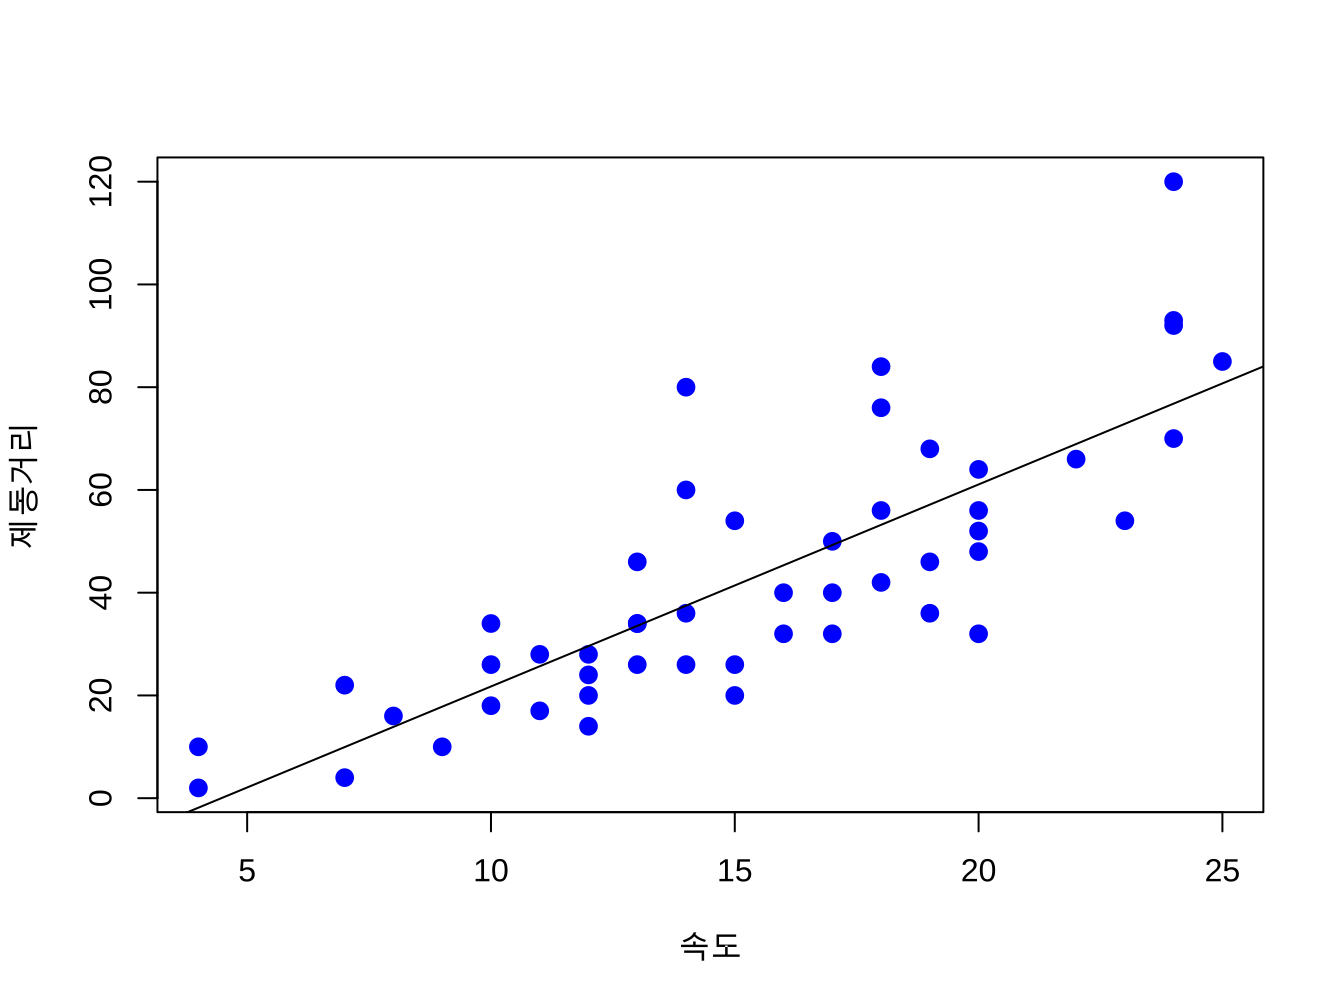
\includegraphics[width=0.8\linewidth]{bookdownintro_files/figure-latex/fig1-1} 

}

\caption{속도와 제동 거리간의 관계}\label{fig:fig1}
\end{figure}

다음 그림은 다음의 chunk 선택문을 이용한 그림이다.

\begin{verbatim}
 out.width='50%', fig.asp=1.25 , fig.align='left'
\end{verbatim}

\begin{Shaded}
\begin{Highlighting}[]
\FunctionTok{plot}\NormalTok{(cars, }\AttributeTok{pch =} \DecValTok{16}\NormalTok{, }\AttributeTok{cex =} \FloatTok{1.3}\NormalTok{, }\AttributeTok{col =} \StringTok{"blue"}\NormalTok{, }\AttributeTok{xlab =} \StringTok{"속도"}\NormalTok{, }\AttributeTok{ylab =} \StringTok{"제동거리"}\NormalTok{)}
\FunctionTok{abline}\NormalTok{(}\FunctionTok{lm}\NormalTok{(dist }\SpecialCharTok{\textasciitilde{}}\NormalTok{ speed, }\AttributeTok{data =}\NormalTok{ cars))}
\end{Highlighting}
\end{Shaded}

\begin{figure}

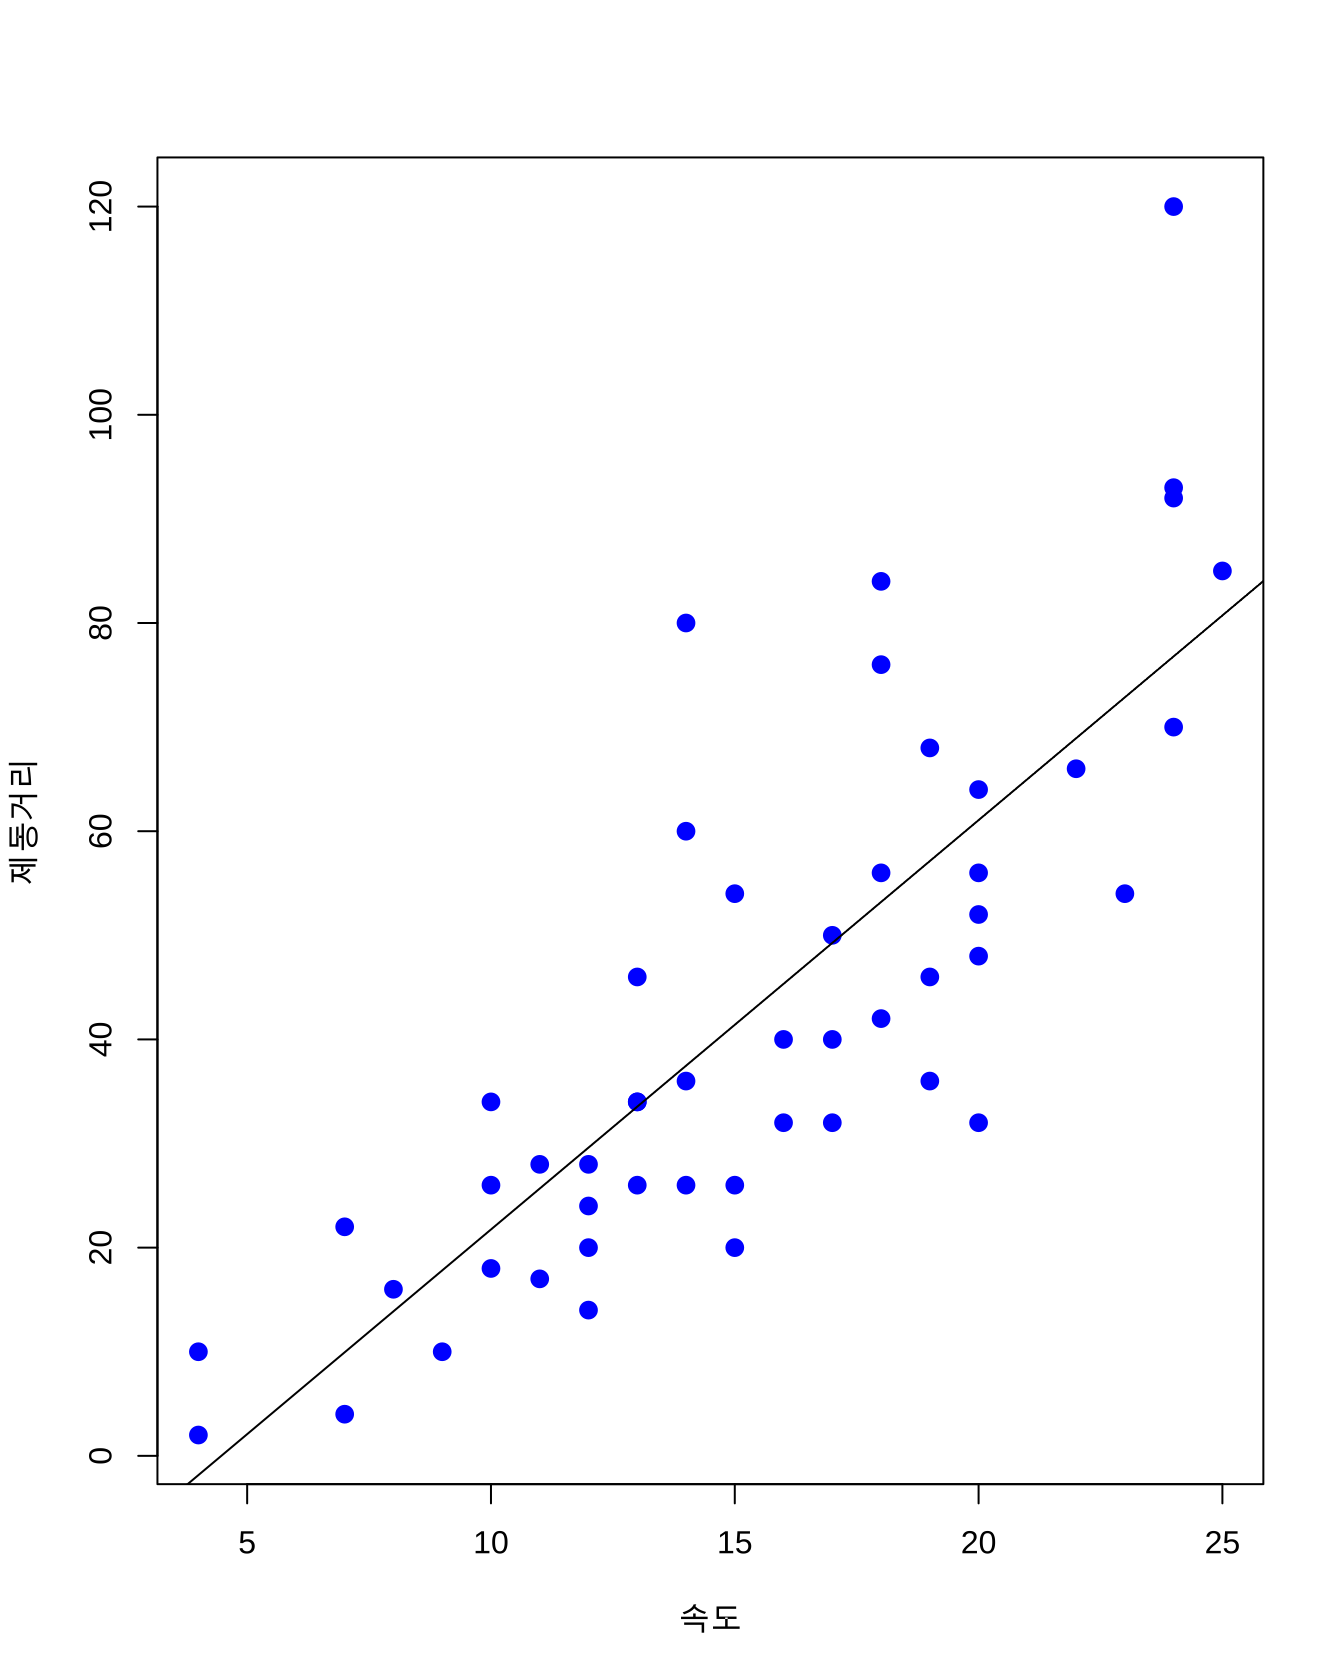
\includegraphics[width=0.5\linewidth]{bookdownintro_files/figure-latex/fig11-1} \hfill{}

\caption{속도와 제동 거리간의 관계}\label{fig:fig11}
\end{figure}

\hypertarget{uxadf8uxb9bc-uxd654uxc77c}{%
\section{그림 화일}\label{uxadf8uxb9bc-uxd654uxc77c}}

화일로 된 그림을 불러오는 방법은 두 가지가 있다. Markdown 명령문을 사용하는 방법과 \texttt{R} 명령문 \texttt{knitr::include\_graphics} 을 사용할 수 있다.

참고로 그림 라벨을 지정하거나 크기를 바꾸는 작업은 Markdown 명령문을을 이용하는 것보다 R 명령문 \texttt{knitr::include\_graphics} 을 사용하는 것이 더 편리하다.

그림 화일 \texttt{f35.jpg} 이 프로젝트 디렉토리 아래 \texttt{myimages/} 디렉토리에 저장되어 있다고 하자 (그림출처:\url{https://rokaf.airforce.mil.kr/})

\hypertarget{r-uxba85uxb839uxbb38uxc758-uxc0acuxc6a9}{%
\subsection{\texorpdfstring{\texttt{R} 명령문의 사용}{R 명령문의 사용}}\label{r-uxba85uxb839uxbb38uxc758-uxc0acuxc6a9}}

\texttt{R} 명령문 \texttt{knitr::include\_graphics}을 사용하여 그림화일을 불러올 수 있다. 이때 사용되는
중요한 chunk 명령어는 다음과 같다.

\begin{itemize}
\tightlist
\item
  \texttt{out.width="50\%"} : 그림의 크기 조절
\item
  \texttt{fig.asp=.75} : 높이/폭의 상대적인 비율
\item
  \texttt{fig.align=\textquotesingle{}center\textquotesingle{}} 그림의 위치
\item
  \texttt{fig.cap=\textquotesingle{}그림\ 제목\textquotesingle{}} : 그림의 제목
\end{itemize}

\begin{verbatim}
knitr::include_graphics("myimages/f35.jpg"))
\end{verbatim}

\begin{Shaded}
\begin{Highlighting}[]
\NormalTok{knitr}\SpecialCharTok{::}\FunctionTok{include\_graphics}\NormalTok{(}\StringTok{"myimages/f35.jpg"}\NormalTok{)}
\end{Highlighting}
\end{Shaded}

\begin{figure}

{\centering 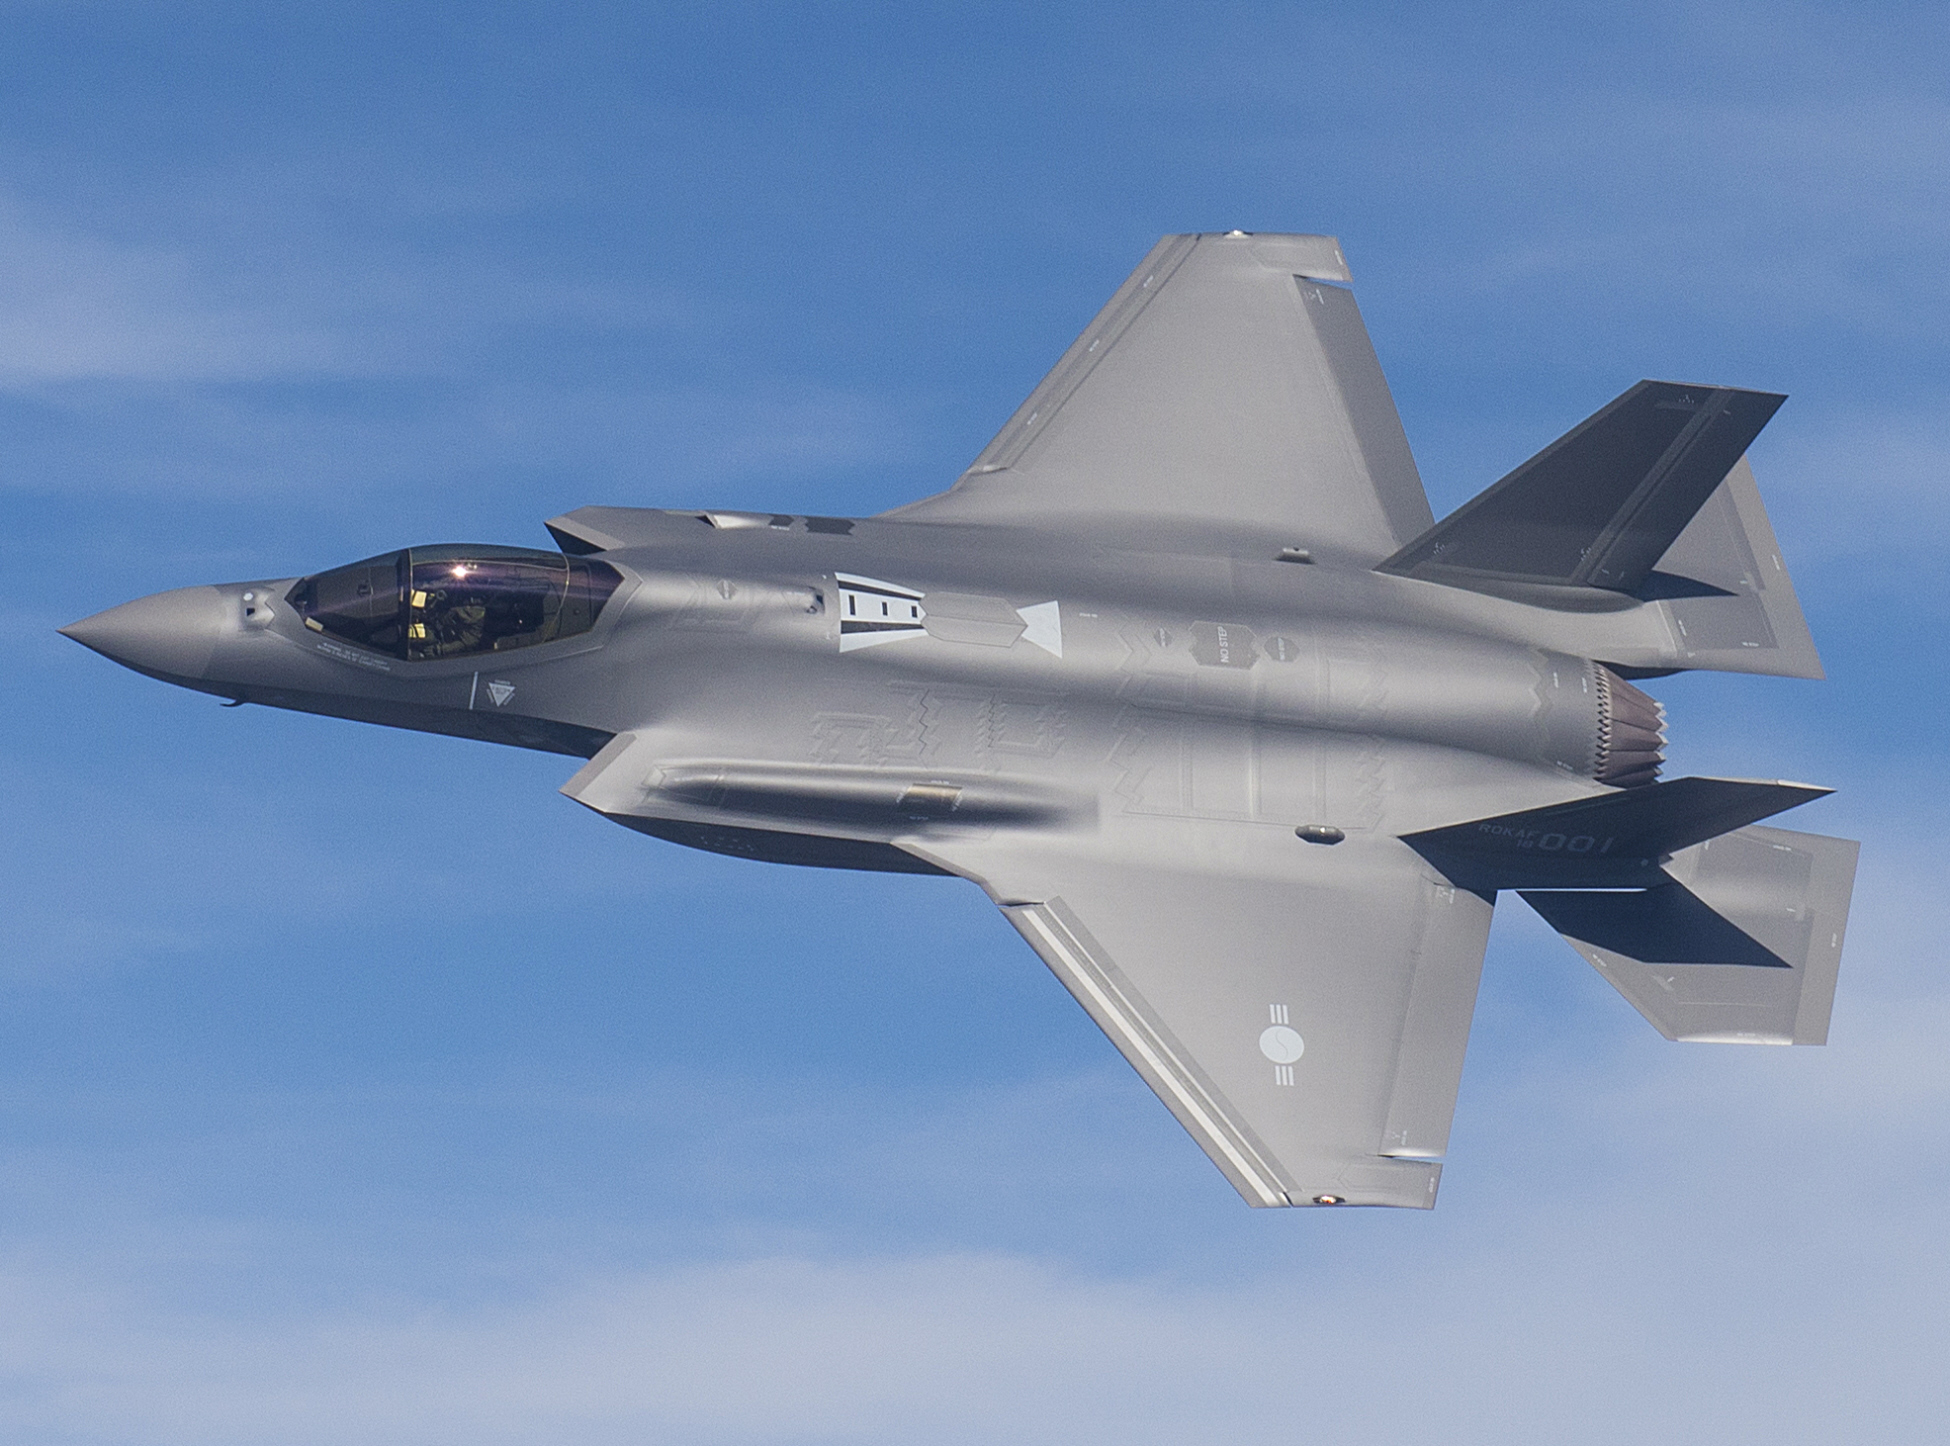
\includegraphics[width=0.8\linewidth]{myimages/f35} 

}

\caption{한국공군 F-35A}\label{fig:f35a}
\end{figure}

\hypertarget{markdown-uxba85uxb839uxbb38uxc758-uxc0acuxc6a9}
\end{verbatim}

\begin{figure}
\centering
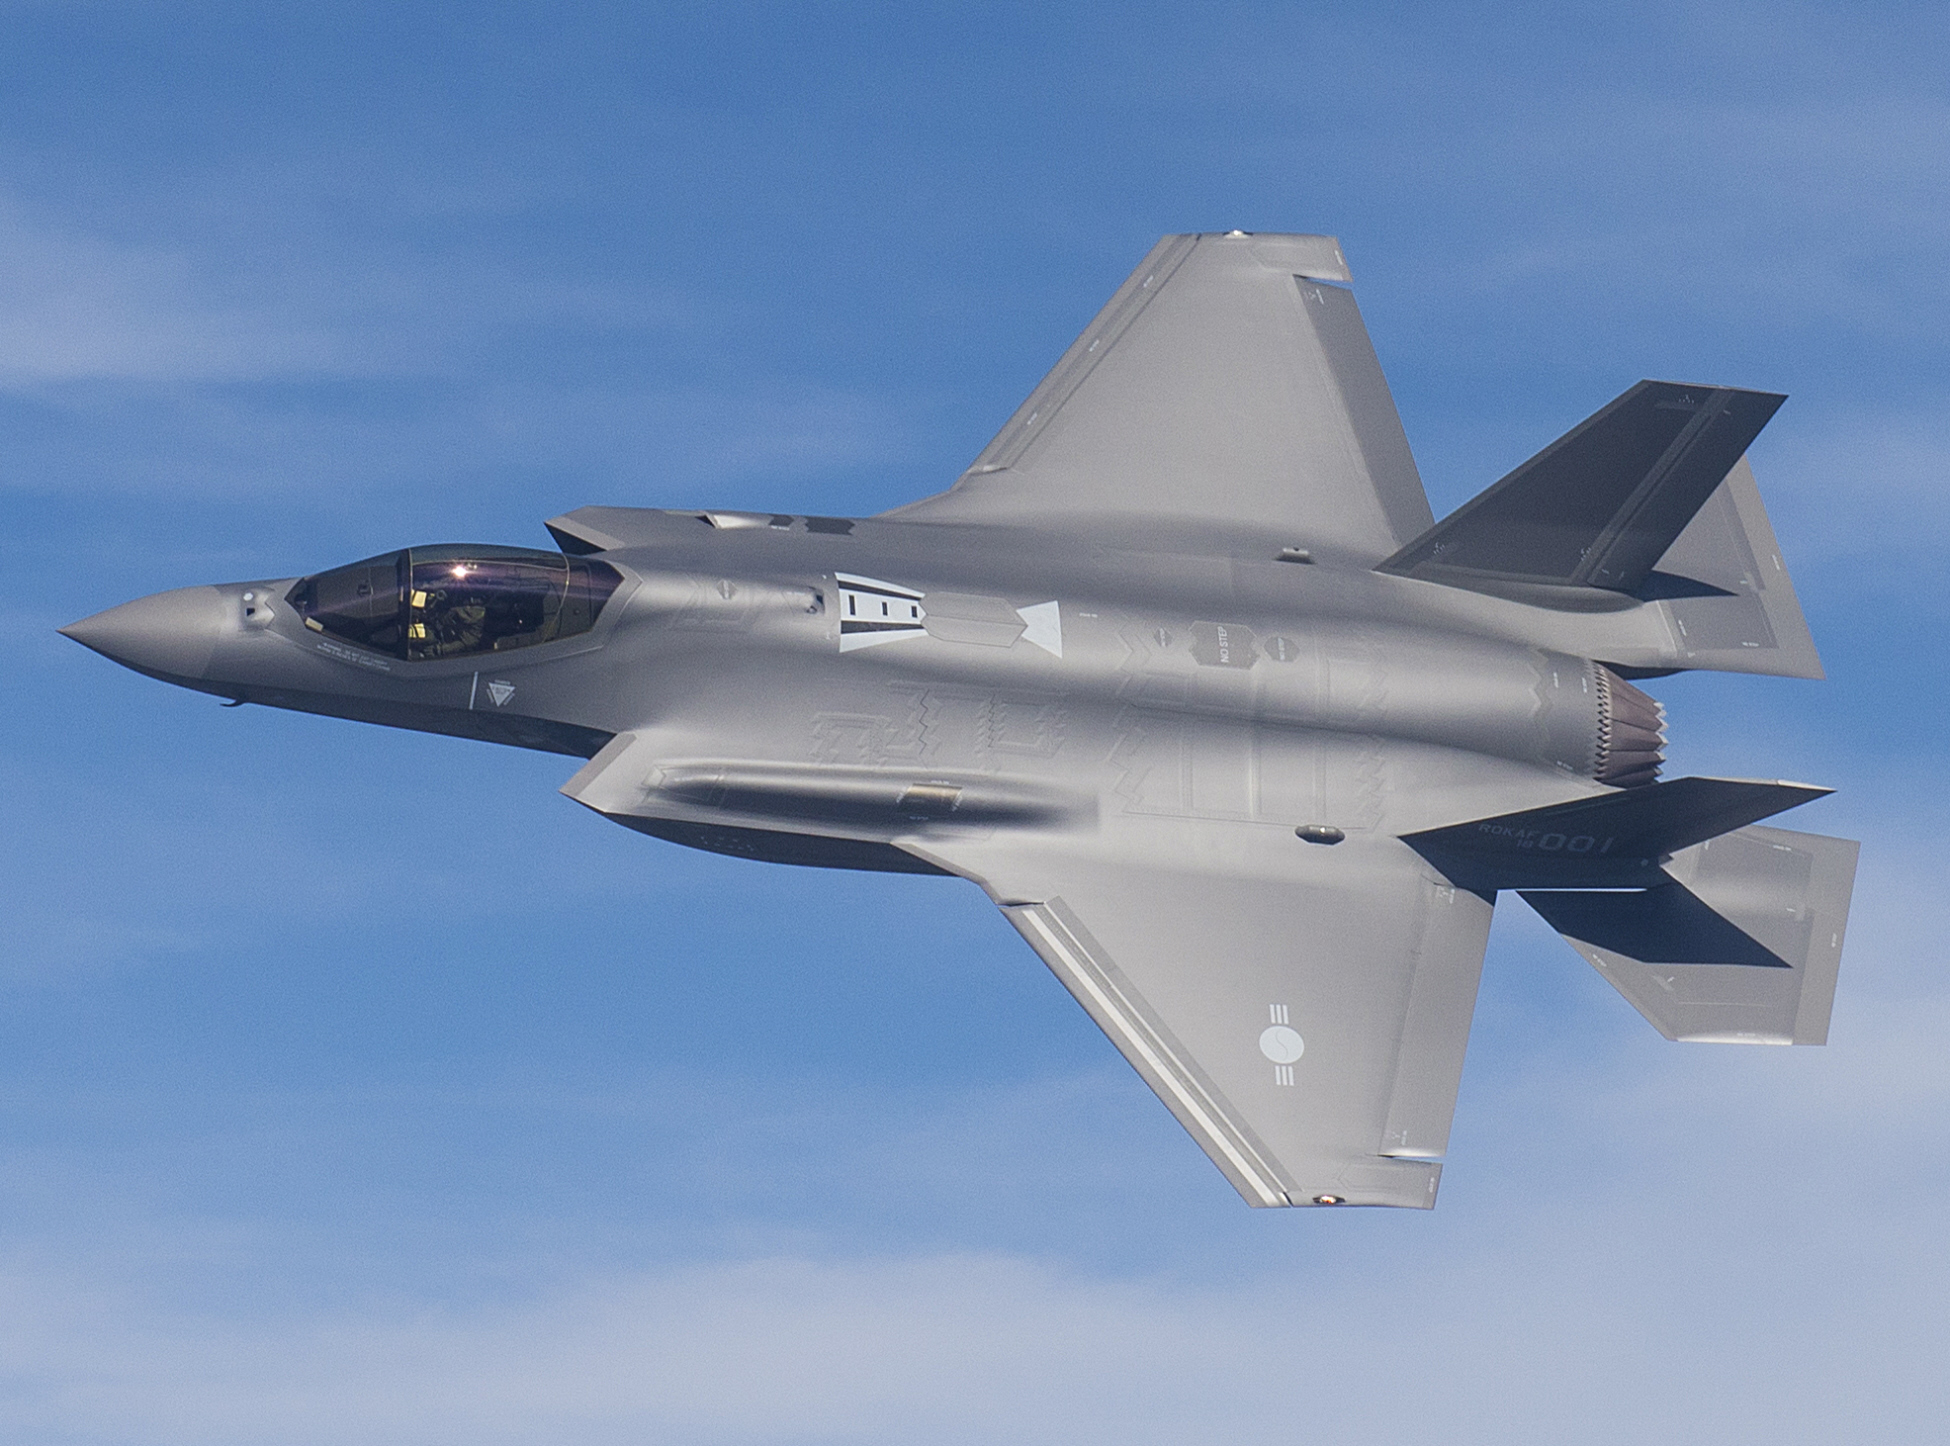
\includegraphics[width=0.5\textwidth,height=\textheight]{myimages/f35.jpg}
\caption{한국공군 F-35A}
\end{figure}

\hypertarget{uxadf8uxb9bcuxc758-uxcc38uxc870}{%
\section{그림의 참조}\label{uxadf8uxb9bcuxc758-uxcc38uxc870}}

그림을 참조하는 경우 chunk 명령문에 사용한 그림 이름 앞에 \texttt{fig:} 를 붙여서 \texttt{\textbackslash{}@ref(fig:figname)} 과 같이 참조한다.

예를 들면 그림 \ref{fig:f35a} 에 나타난 비행기는 한국 공군의 F-35A 이다.

\hypertarget{uxac1c-uxc774uxc0c1uxc758-uxadf8uxb9bc}{%
\section{2개 이상의 그림}\label{uxac1c-uxc774uxc0c1uxc758-uxadf8uxb9bc}}

하나의 화면에 두 개 이상의 그림을 그리려면 chunk 명령문에 \texttt{fig.show\ =\ \textquotesingle{}hold\textquotesingle{}} 을 추가한다.

\begin{Shaded}
\begin{Highlighting}[]
\FunctionTok{par}\NormalTok{(}\AttributeTok{mar =} \FunctionTok{c}\NormalTok{(}\DecValTok{4}\NormalTok{, }\DecValTok{4}\NormalTok{, .}\DecValTok{1}\NormalTok{, .}\DecValTok{1}\NormalTok{))}
\NormalTok{knitr}\SpecialCharTok{::}\FunctionTok{include\_graphics}\NormalTok{(}\StringTok{"myimages/f35.jpg"}\NormalTok{)}
\FunctionTok{plot}\NormalTok{(cars, }\AttributeTok{pch =} \DecValTok{16}\NormalTok{, }\AttributeTok{cex =} \FloatTok{1.3}\NormalTok{, }\AttributeTok{col =} \StringTok{"blue"}\NormalTok{, }\AttributeTok{xlab=}\StringTok{"속도"}\NormalTok{, }\AttributeTok{ylab=}\StringTok{"제동거리"}\NormalTok{)}
\FunctionTok{abline}\NormalTok{(}\FunctionTok{lm}\NormalTok{(dist }\SpecialCharTok{\textasciitilde{}}\NormalTok{ speed, }\AttributeTok{data=}\NormalTok{cars))}
\end{Highlighting}
\end{Shaded}

\begin{figure}
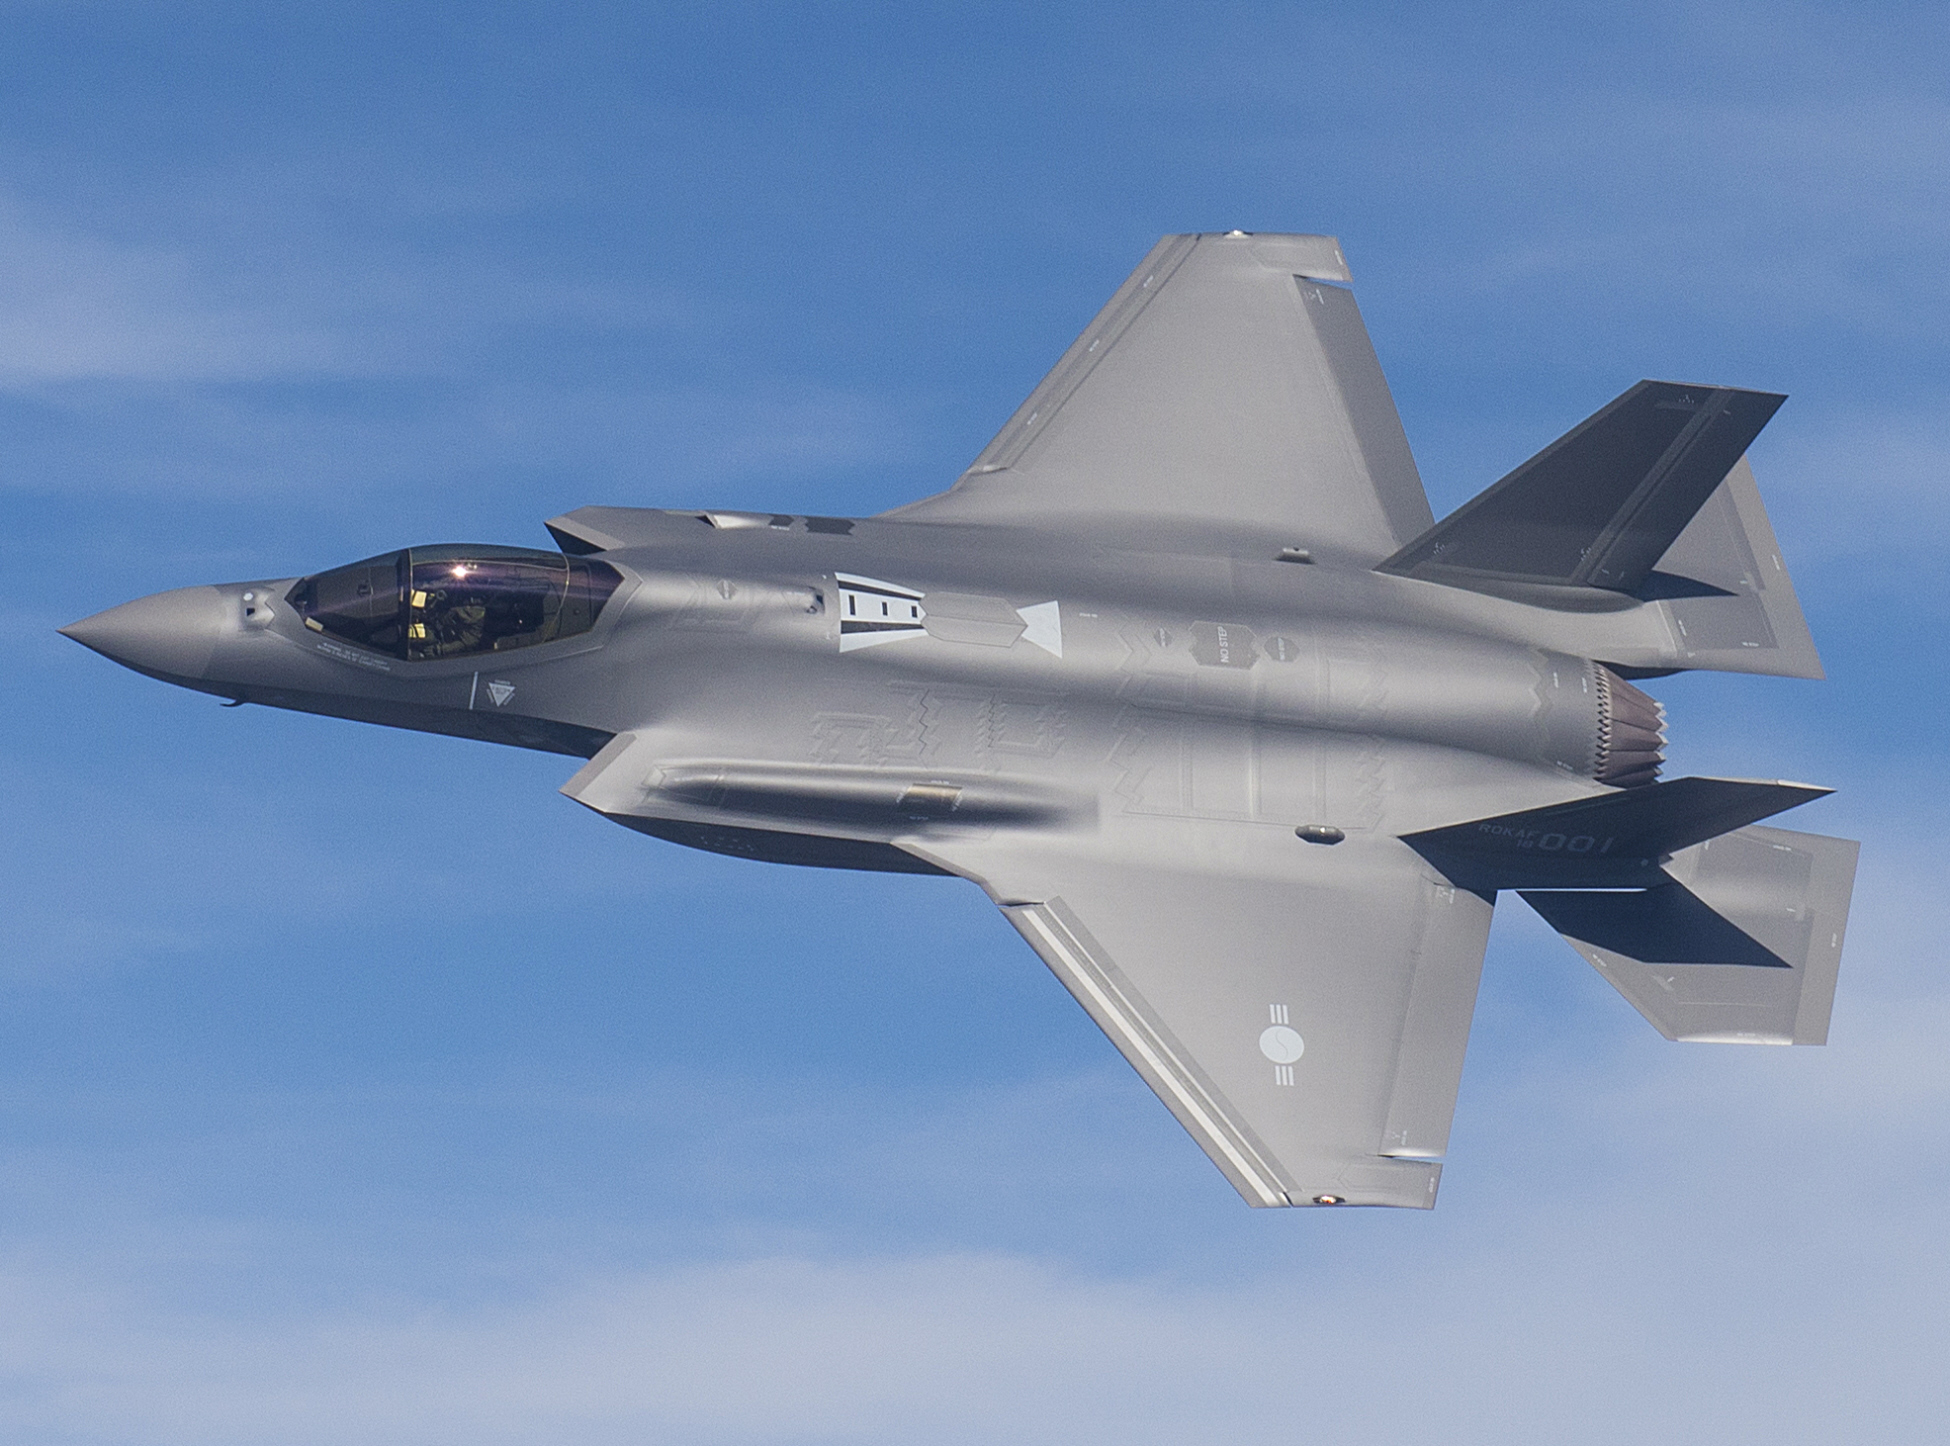
\includegraphics[width=0.5\linewidth]{myimages/f35} 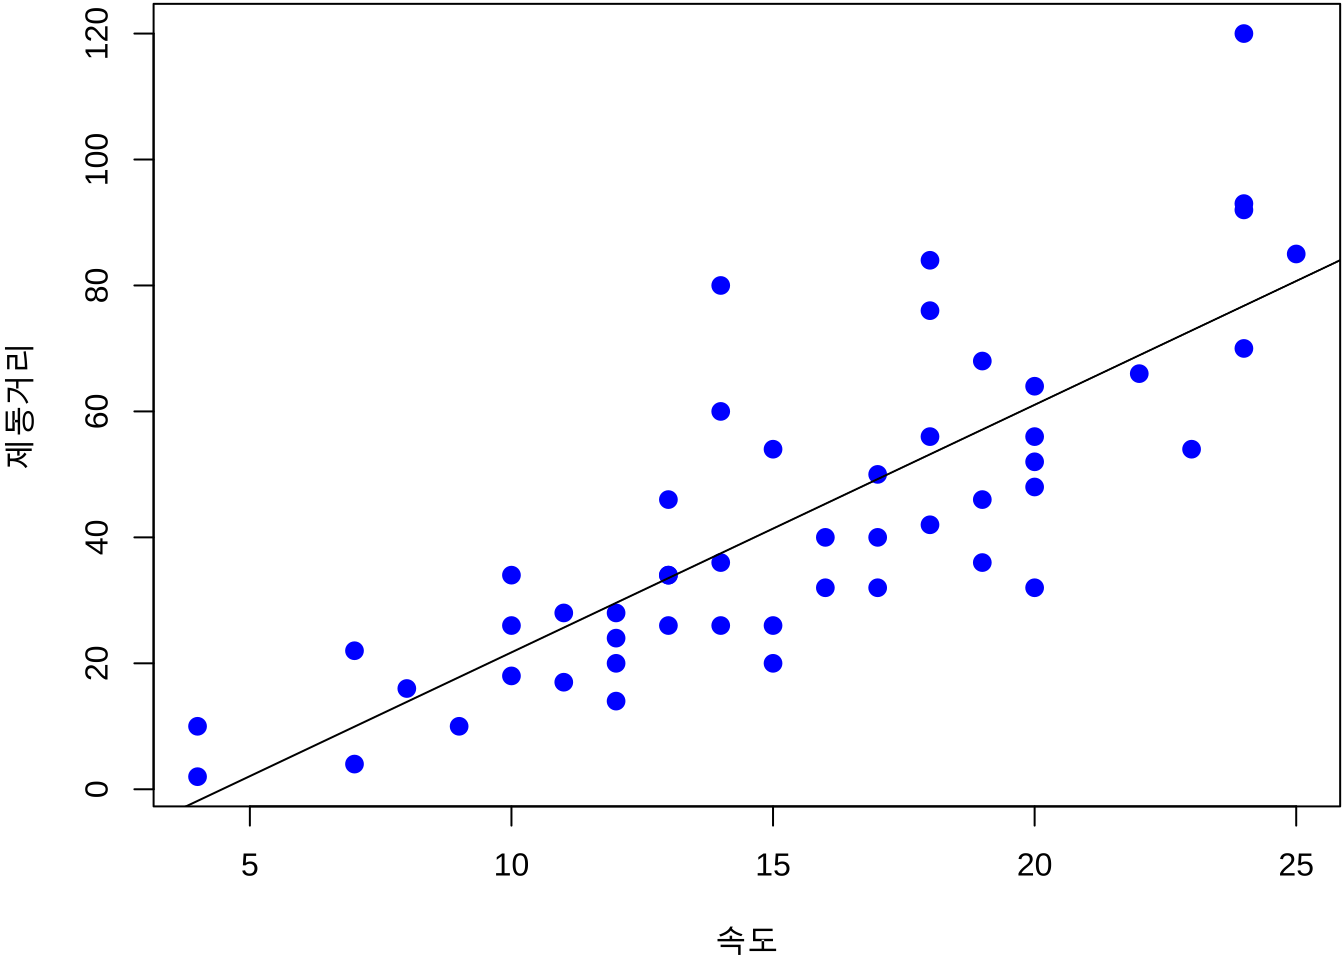
\includegraphics[width=0.5\linewidth]{bookdownintro_files/figure-latex/twoplots-2} \caption{동시에 두 개의 그림 그리기}\label{fig:twoplots}
\end{figure}

다음과 같이 \texttt{ggplot2} 와 \texttt{plot} 함수를 이용하여 2 개의 그림을 같이 그릴 수 있다.

\begin{Shaded}
\begin{Highlighting}[]
\FunctionTok{par}\NormalTok{(}\AttributeTok{mar =} \FunctionTok{c}\NormalTok{(}\DecValTok{4}\NormalTok{, }\DecValTok{4}\NormalTok{, .}\DecValTok{1}\NormalTok{, .}\DecValTok{1}\NormalTok{))}
\FunctionTok{ggplot}\NormalTok{(cars,  }\FunctionTok{aes}\NormalTok{(}\AttributeTok{x=}\NormalTok{speed, }\AttributeTok{y=}\NormalTok{dist)) }\SpecialCharTok{+} \FunctionTok{geom\_point}\NormalTok{() }\SpecialCharTok{+} \FunctionTok{geom\_smooth}\NormalTok{(}\AttributeTok{method =} \StringTok{"lm"}\NormalTok{, }\AttributeTok{se =} \ConstantTok{FALSE}\NormalTok{) }\SpecialCharTok{+} \FunctionTok{labs}\NormalTok{(}\AttributeTok{x =} \StringTok{"속도"}\NormalTok{, }\AttributeTok{y =} \StringTok{"거리"}\NormalTok{)  }\SpecialCharTok{+} \FunctionTok{theme\_bw}\NormalTok{()}
\FunctionTok{plot}\NormalTok{(cars, }\AttributeTok{pch =} \DecValTok{16}\NormalTok{, }\AttributeTok{cex =} \FloatTok{1.3}\NormalTok{, }\AttributeTok{col =} \StringTok{"blue"}\NormalTok{, }\AttributeTok{xlab=}\StringTok{"속도"}\NormalTok{, }\AttributeTok{ylab=}\StringTok{"제동거리"}\NormalTok{)}
\FunctionTok{abline}\NormalTok{(}\FunctionTok{lm}\NormalTok{(dist }\SpecialCharTok{\textasciitilde{}}\NormalTok{ speed, }\AttributeTok{data=}\NormalTok{cars))}
\end{Highlighting}
\end{Shaded}

\begin{figure}
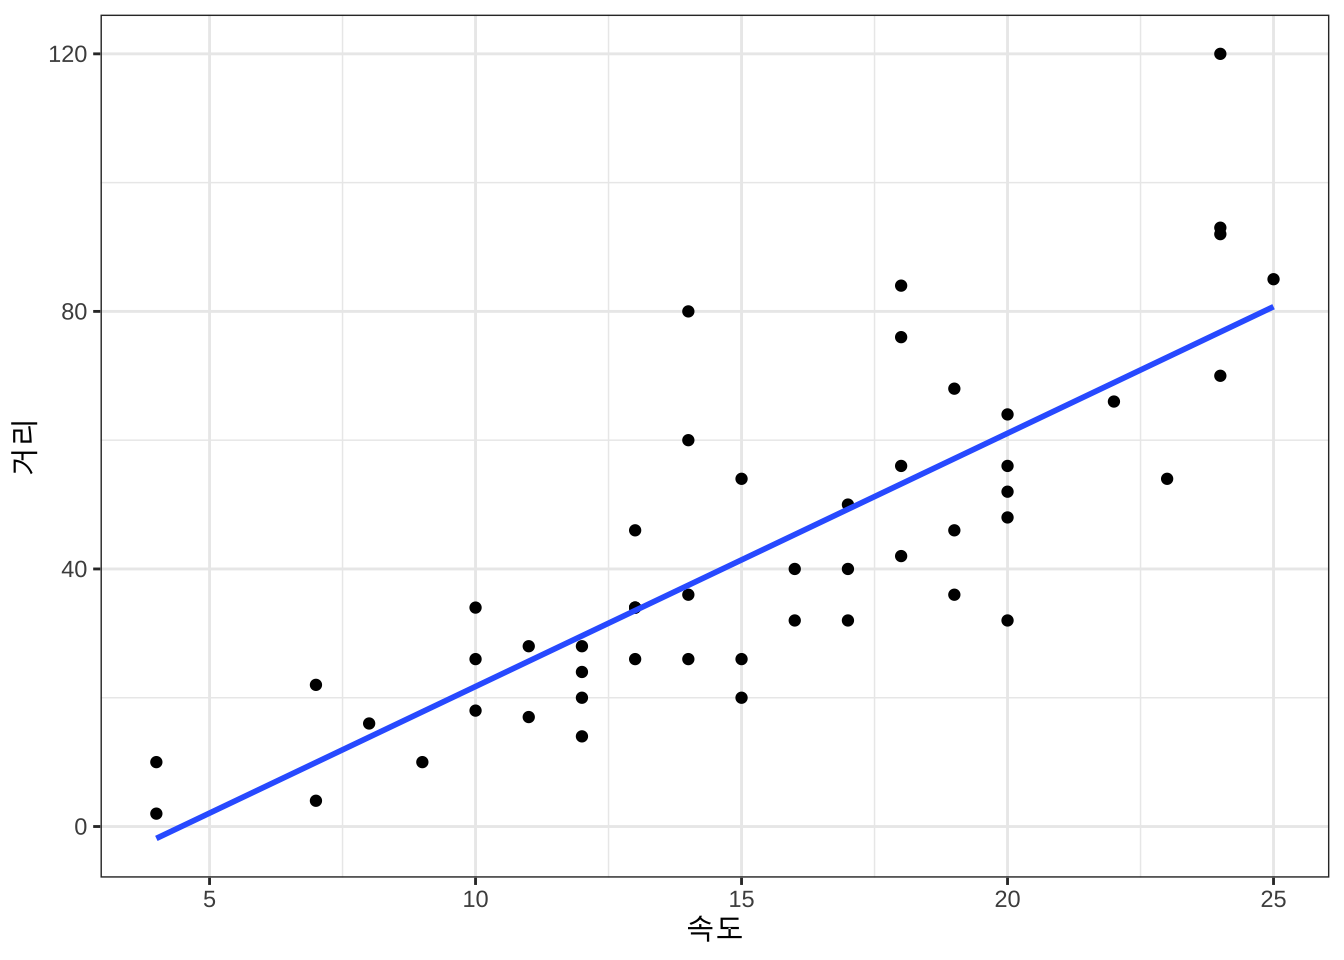
\includegraphics[width=0.5\linewidth]{bookdownintro_files/figure-latex/twoplots2-1} 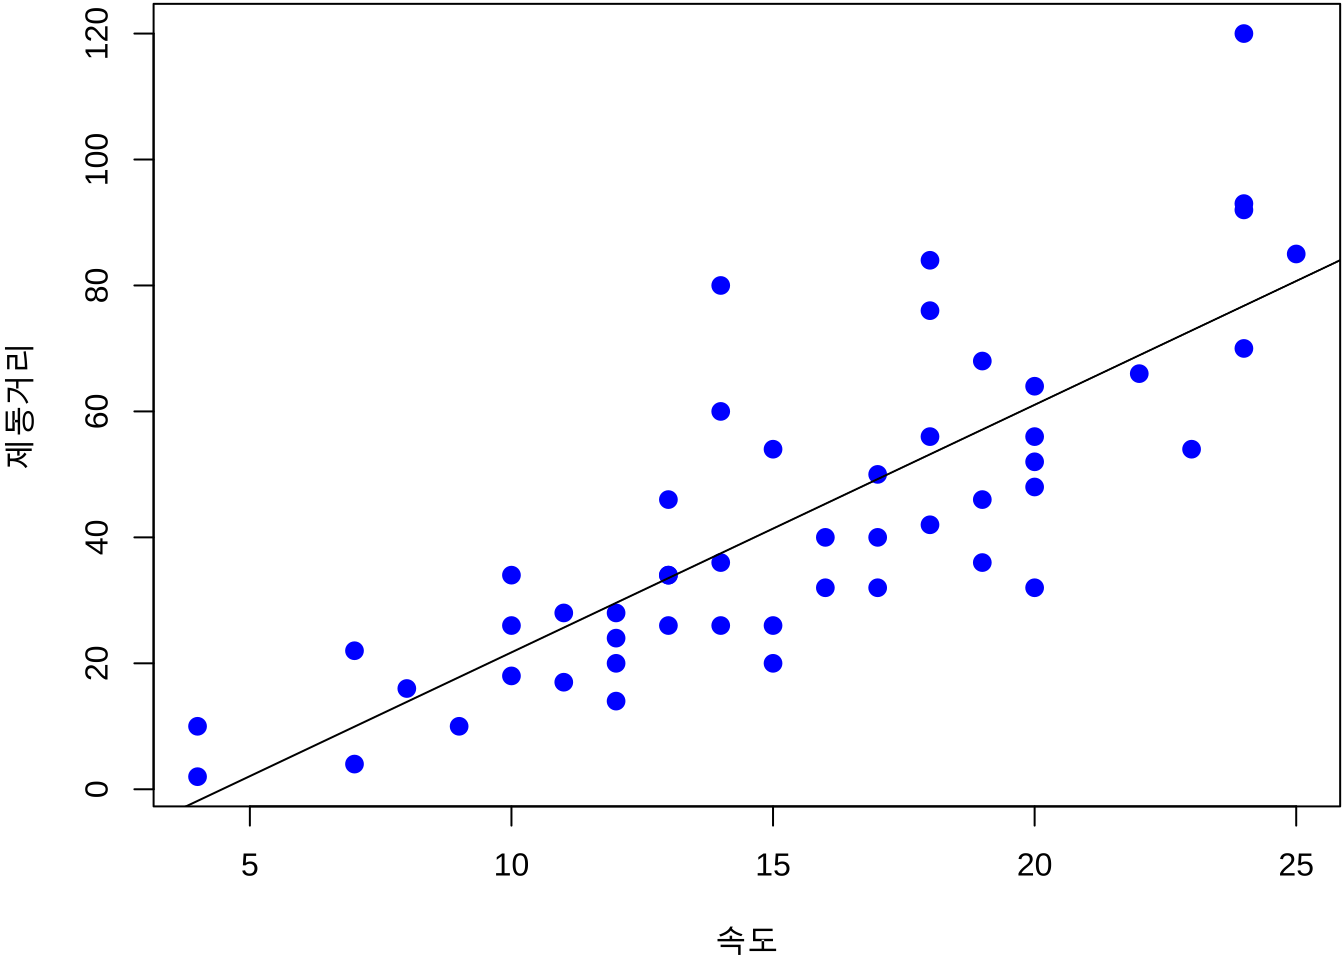
\includegraphics[width=0.5\linewidth]{bookdownintro_files/figure-latex/twoplots2-2} \caption{ggplot2 와 plot}\label{fig:twoplots2}
\end{figure}

\hypertarget{uxd328uxd0a4uxc9c0-ggplot2-uxc608uxc81c}{%
\section{\texorpdfstring{패키지 \texttt{ggplot2} 예제}{패키지 ggplot2 예제}}\label{uxd328uxd0a4uxc9c0-ggplot2-uxc608uxc81c}}

패키지 \texttt{ggplot2} 를 이용한 그림도 다음과 같이 나타낼 수 있다.

\begin{Shaded}
\begin{Highlighting}[]
\FunctionTok{ggplot}\NormalTok{(cars, }\FunctionTok{aes}\NormalTok{(}\AttributeTok{x =}\NormalTok{ speed, }\AttributeTok{y =}\NormalTok{ dist)) }\SpecialCharTok{+} \FunctionTok{geom\_point}\NormalTok{() }\SpecialCharTok{+} \FunctionTok{geom\_smooth}\NormalTok{(}\AttributeTok{method =} \StringTok{"lm"}\NormalTok{, }
    \AttributeTok{se =} \ConstantTok{FALSE}\NormalTok{) }\SpecialCharTok{+} \FunctionTok{labs}\NormalTok{(}\AttributeTok{x =} \StringTok{"속도"}\NormalTok{, }\AttributeTok{y =} \StringTok{"거리"}\NormalTok{) }\SpecialCharTok{+} \FunctionTok{theme\_bw}\NormalTok{()}
\end{Highlighting}
\end{Shaded}

\begin{verbatim}
## `geom_smooth()` using formula 'y ~ x'
\end{verbatim}

\begin{center}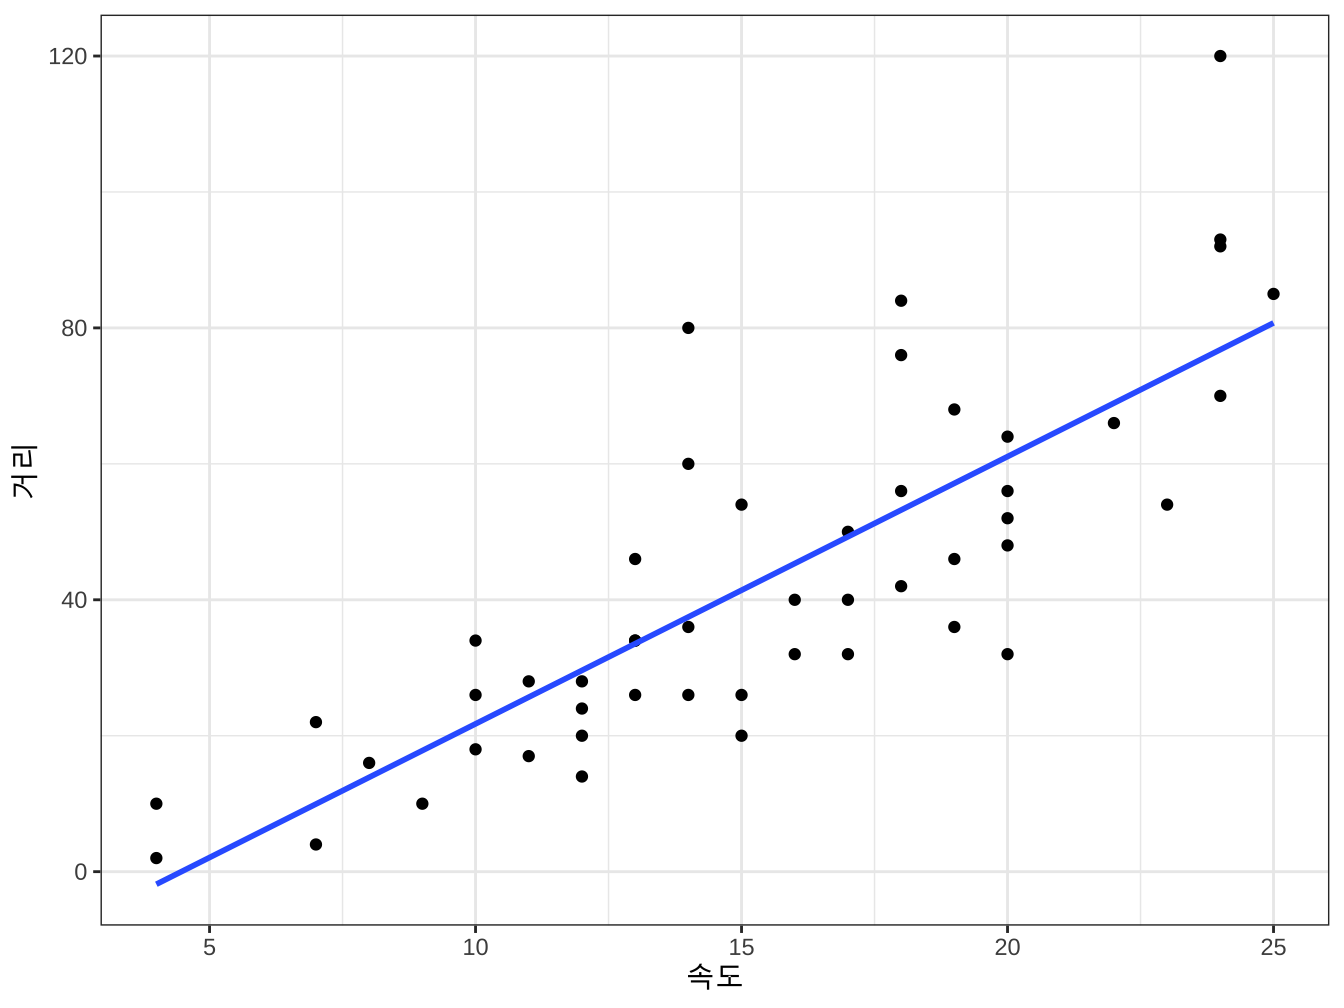
\includegraphics[width=0.6\linewidth]{bookdownintro_files/figure-latex/fig2-1} \end{center}

\begin{Shaded}
\begin{Highlighting}[]
\FunctionTok{ggplot}\NormalTok{(mtcars, }\FunctionTok{aes}\NormalTok{(wt, mpg)) }\SpecialCharTok{+} \FunctionTok{geom\_point}\NormalTok{(}\FunctionTok{aes}\NormalTok{(}\AttributeTok{colour =} \FunctionTok{factor}\NormalTok{(cyl)), }\AttributeTok{size =} \DecValTok{2}\NormalTok{) }\SpecialCharTok{+} 
    \FunctionTok{labs}\NormalTok{(}\AttributeTok{x =} \StringTok{"무게"}\NormalTok{, }\AttributeTok{y =} \StringTok{"마일리지"}\NormalTok{, }\AttributeTok{color =} \StringTok{"실린더 개수"}\NormalTok{) }\SpecialCharTok{+} \FunctionTok{theme\_bw}\NormalTok{()}
\end{Highlighting}
\end{Shaded}

\begin{center}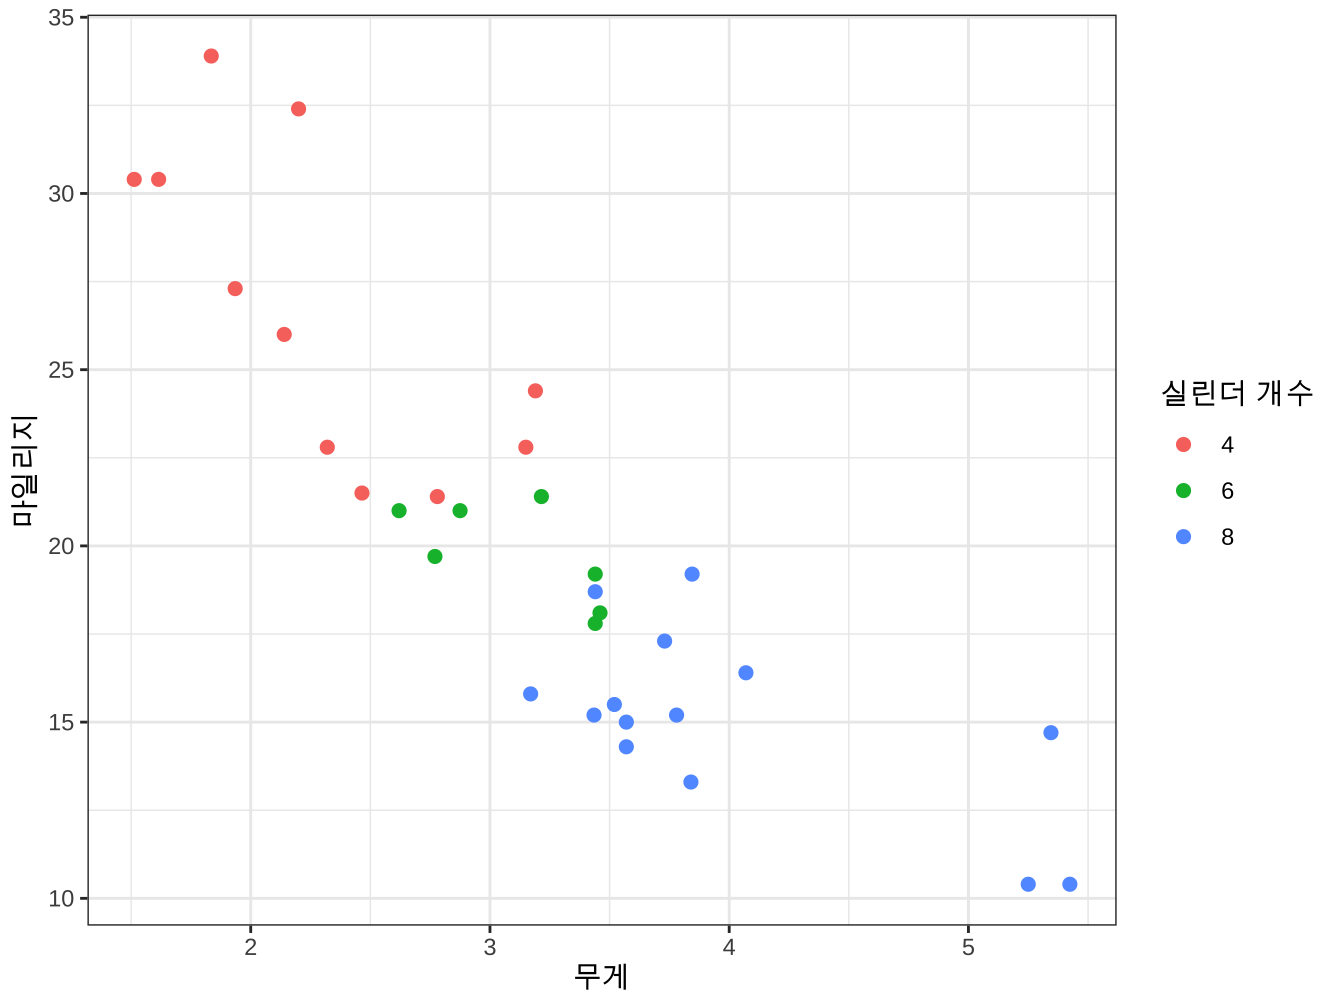
\includegraphics[width=0.8\linewidth]{bookdownintro_files/figure-latex/fig21-1} \end{center}

\begin{Shaded}
\begin{Highlighting}[]
\FunctionTok{ggplot}\NormalTok{(mpg, }\FunctionTok{aes}\NormalTok{(displ, hwy)) }\SpecialCharTok{+} \FunctionTok{geom\_point}\NormalTok{(}\AttributeTok{size =} \FloatTok{0.8}\NormalTok{) }\SpecialCharTok{+} \FunctionTok{facet\_wrap}\NormalTok{(}\FunctionTok{vars}\NormalTok{(class)) }\SpecialCharTok{+} 
    \FunctionTok{labs}\NormalTok{(}\AttributeTok{x =} \StringTok{"무게"}\NormalTok{, }\AttributeTok{y =} \StringTok{"마일리지"}\NormalTok{) }\SpecialCharTok{+} \FunctionTok{theme\_bw}\NormalTok{()}
\end{Highlighting}
\end{Shaded}

\begin{center}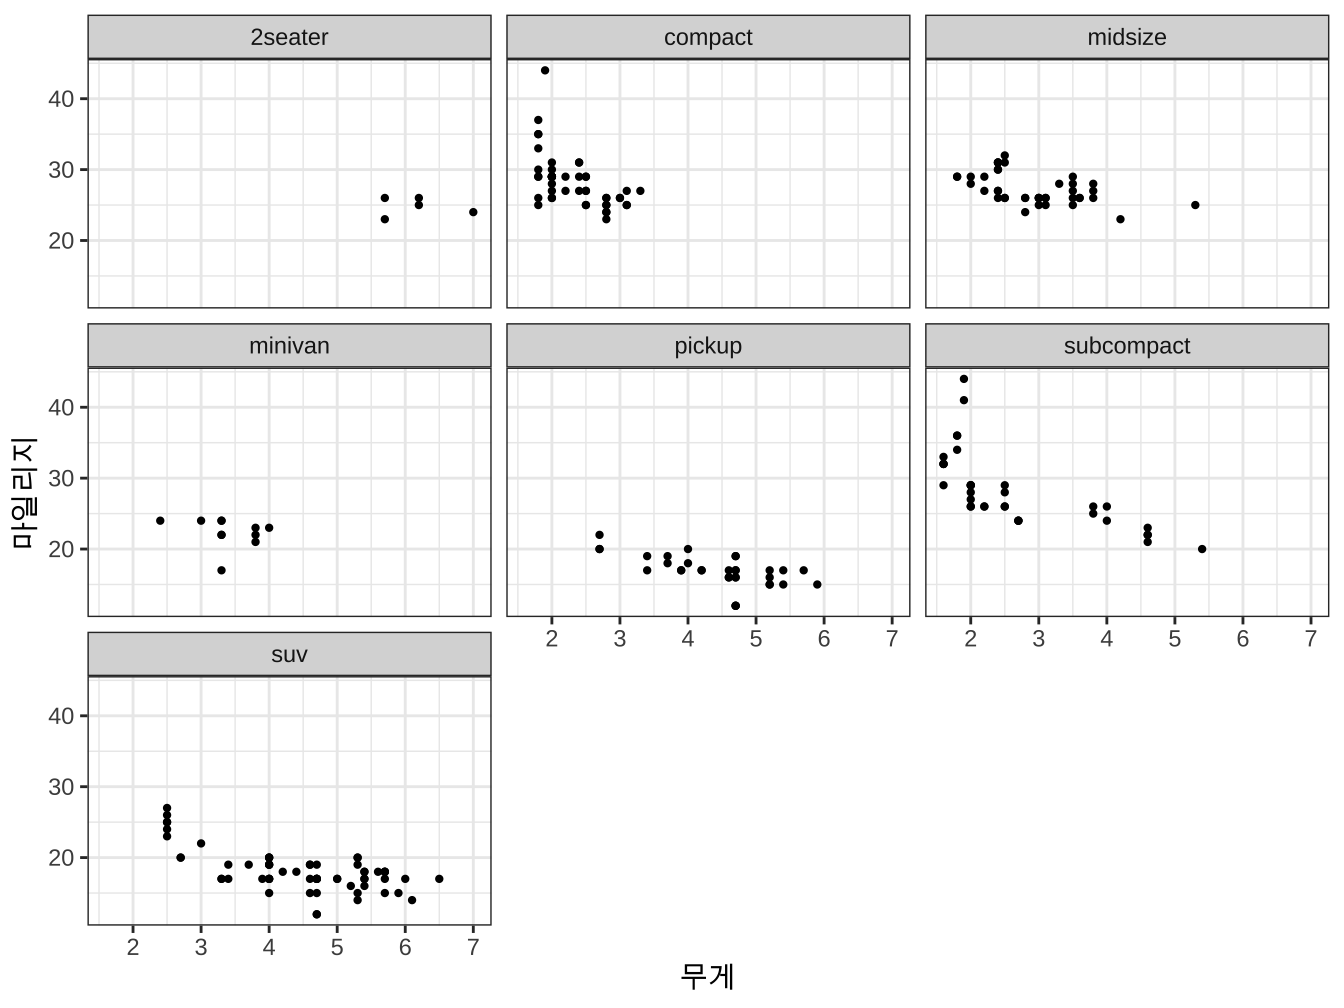
\includegraphics[width=0.8\linewidth]{bookdownintro_files/figure-latex/fig22-1} \end{center}

\hypertarget{table}{%
\chapter{표}\label{table}}

\hypertarget{kable-uxd568uxc218}{%
\section{\texorpdfstring{\texttt{kable} 함수}{kable 함수}}\label{kable-uxd568uxc218}}

\texttt{knitr} 패키지의 \texttt{kable} 함수를 이용하면 데이터프레임을 표 형식으로 표시할 수 있다.

\begin{Shaded}
\begin{Highlighting}[]
\NormalTok{knitr}\SpecialCharTok{::}\FunctionTok{kable}\NormalTok{(}
  \FunctionTok{head}\NormalTok{(iris, }\DecValTok{5}\NormalTok{), }\AttributeTok{caption =} \StringTok{\textquotesingle{}kable 로 만든 표\textquotesingle{}}\NormalTok{,}
  \AttributeTok{booktabs =} \ConstantTok{TRUE}\NormalTok{,}
  \AttributeTok{digits =} \DecValTok{2}
\NormalTok{)}
\end{Highlighting}
\end{Shaded}

\begin{table}

\caption{\label{tab:tble1}kable 로 만든 표}
\centering
\begin{tabular}[t]{rrrrl}
\toprule
Sepal.Length & Sepal.Width & Petal.Length & Petal.Width & Species\\
\midrule
5.1 & 3.5 & 1.4 & 0.2 & setosa\\
4.9 & 3.0 & 1.4 & 0.2 & setosa\\
4.7 & 3.2 & 1.3 & 0.2 & setosa\\
4.6 & 3.1 & 1.5 & 0.2 & setosa\\
5.0 & 3.6 & 1.4 & 0.2 & setosa\\
\bottomrule
\end{tabular}
\end{table}

\hypertarget{kableextra-uxd328uxd0a4uxc9c0}{%
\section{\texorpdfstring{\texttt{kableExtra} 패키지}{kableExtra 패키지}}\label{kableextra-uxd328uxd0a4uxc9c0}}

\texttt{kableExtra} 패키지는 더 다양한 형식의 표를 만들 수 있다.

\begin{Shaded}
\begin{Highlighting}[]
\FunctionTok{head}\NormalTok{(iris, }\DecValTok{5}\NormalTok{) }\SpecialCharTok{\%\textgreater{}\%}
  \FunctionTok{kbl}\NormalTok{(}\AttributeTok{caption =} \StringTok{\textquotesingle{}kableExtra 로 만든 표\textquotesingle{}}\NormalTok{) }\SpecialCharTok{\%\textgreater{}\%}
  \FunctionTok{kable\_styling}\NormalTok{(}\AttributeTok{bootstrap\_options =} \StringTok{"striped"}\NormalTok{, }\AttributeTok{full\_width =}\NormalTok{ F, }\AttributeTok{position =} \StringTok{"center"}\NormalTok{, }\AttributeTok{font\_size =} \DecValTok{11}\NormalTok{)}
\end{Highlighting}
\end{Shaded}

\begin{table}

\caption{\label{tab:tbl2}kableExtra 로 만든 표}
\centering
\fontsize{11}{13}\selectfont
\begin{tabular}[t]{r|r|r|r|l}
\hline
Sepal.Length & Sepal.Width & Petal.Length & Petal.Width & Species\\
\hline
5.1 & 3.5 & 1.4 & 0.2 & setosa\\
\hline
4.9 & 3.0 & 1.4 & 0.2 & setosa\\
\hline
4.7 & 3.2 & 1.3 & 0.2 & setosa\\
\hline
4.6 & 3.1 & 1.5 & 0.2 & setosa\\
\hline
5.0 & 3.6 & 1.4 & 0.2 & setosa\\
\hline
\end{tabular}
\end{table}

\texttt{kableExtra} 패키지의 자세한 이용법은 \href{https://cran.r-project.org/web/packages/kableExtra/vignettes/awesome_table_in_html.html}{매뉴얼} 에서 찾을 수 있다.

\hypertarget{markdown-uxd45c}{%
\section{\texorpdfstring{\texttt{markdown} 표}{markdown 표}}\label{markdown-uxd45c}}

\texttt{markdown} 형식을 이용하여 직접 표를 작성할 수 있다.

\begin{Shaded}
\begin{Highlighting}[]
\NormalTok{| 환자 번호  | Treatment  | Value |}
\NormalTok{|{-}{-}{-}{-}{-}{-}:|:{-}{-}{-}{-}{-}{-}:|:{-}{-}{-}{-}{-}{-}{-}{-}{-}{-}|}
\NormalTok{|   1   |   a    | $\textbackslash{}alpha$  |}
\NormalTok{|   2   |   b    | $\textbackslash{}beta$   |}
\NormalTok{|   3   |   b    | $\textbackslash{}gamma$  |}


\NormalTok{: (}\SpecialCharTok{\textbackslash{}\#}\NormalTok{tab:marktable) 마크다운 테이블 }
\end{Highlighting}
\end{Shaded}

\begin{longtable}[]{@{}rcl@{}}
\caption{\label{tab:marktable} 마크다운 테이블}\tabularnewline
\toprule
환자 번호 & Treatment & Value\tabularnewline
\midrule
\endfirsthead
\toprule
환자 번호 & Treatment & Value\tabularnewline
\midrule
\endhead
1 & a & \(\alpha\)\tabularnewline
2 & b & \(\beta\)\tabularnewline
3 & b & \(\gamma\)\tabularnewline
\bottomrule
\end{longtable}

다음과 같이 분산분석표를 markdown 표로 만들 수 있다.

\begin{Shaded}
\begin{Highlighting}[]
\NormalTok{|   요인     |  제곱합  |   자유도   |  평균제곱합    | $F\_0$   |  p{-}값    |}
\NormalTok{|:{-}{-}{-}{-}{-}{-}{-}{-}{-}{-}{-}:|{-}{-}{-}{-}{-}{-}{-}{-}:|{-}{-}{-}{-}{-}{-}{-}{-}{-}{-}{-}:|{-}{-}{-}{-}{-}{-}{-}{-}{-}{-}{-}{-}{-}{-}{-}:|:{-}{-}{-}{-}{-}{-}{-}:|{-}{-}{-}{-}{-}{-}{-}{-}{-}:|}
\NormalTok{|   처리     |  $SS\_A$ |  $\textbackslash{}phi\_A = a{-}1$  |  $MS\_A=SS\_A/\textbackslash{}phi\_A$       | $F\_0=MS\_A/MS\_E$ |  $P}\CommentTok{[}\OtherTok{F(\textbackslash{}phi\_A, \textbackslash{}phi\_E) \textgreater{} F\_0  }\CommentTok{]}\NormalTok{$       |}
\NormalTok{|   잔차   |  $SS\_E$  |  $\textbackslash{}phi\_E=a(r{-}1)$  |  $MS\_E=SS\_E/\textbackslash{}phi\_E$ |  |       |}
\NormalTok{|  총합   |  $SS\_T$  |  $\textbackslash{}phi\_T =  ar{-}1$        |       |        |         |}
\end{Highlighting}
\end{Shaded}

\begin{longtable}[]{@{}crrrcr@{}}
\caption{분산분석표}\tabularnewline
\toprule
\begin{minipage}[b]{(\columnwidth - 5\tabcolsep) * \real{0.19}}\centering
요인\strut
\end{minipage} & \begin{minipage}[b]{(\columnwidth - 5\tabcolsep) * \real{0.13}}\raggedleft
제곱합\strut
\end{minipage} & \begin{minipage}[b]{(\columnwidth - 5\tabcolsep) * \real{0.17}}\raggedleft
자유도\strut
\end{minipage} & \begin{minipage}[b]{(\columnwidth - 5\tabcolsep) * \real{0.23}}\raggedleft
평균제곱합\strut
\end{minipage} & \begin{minipage}[b]{(\columnwidth - 5\tabcolsep) * \real{0.13}}\centering
\(F_0\)\strut
\end{minipage} & \begin{minipage}[b]{(\columnwidth - 5\tabcolsep) * \real{0.14}}\raggedleft
p-값\strut
\end{minipage}\tabularnewline
\midrule
\endfirsthead
\toprule
\begin{minipage}[b]{(\columnwidth - 5\tabcolsep) * \real{0.19}}\centering
요인\strut
\end{minipage} & \begin{minipage}[b]{(\columnwidth - 5\tabcolsep) * \real{0.13}}\raggedleft
제곱합\strut
\end{minipage} & \begin{minipage}[b]{(\columnwidth - 5\tabcolsep) * \real{0.17}}\raggedleft
자유도\strut
\end{minipage} & \begin{minipage}[b]{(\columnwidth - 5\tabcolsep) * \real{0.23}}\raggedleft
평균제곱합\strut
\end{minipage} & \begin{minipage}[b]{(\columnwidth - 5\tabcolsep) * \real{0.13}}\centering
\(F_0\)\strut
\end{minipage} & \begin{minipage}[b]{(\columnwidth - 5\tabcolsep) * \real{0.14}}\raggedleft
p-값\strut
\end{minipage}\tabularnewline
\midrule
\endhead
\begin{minipage}[t]{(\columnwidth - 5\tabcolsep) * \real{0.19}}\centering
처리\strut
\end{minipage} & \begin{minipage}[t]{(\columnwidth - 5\tabcolsep) * \real{0.13}}\raggedleft
\(SS_A\)\strut
\end{minipage} & \begin{minipage}[t]{(\columnwidth - 5\tabcolsep) * \real{0.17}}\raggedleft
\(\phi_A = a-1\)\strut
\end{minipage} & \begin{minipage}[t]{(\columnwidth - 5\tabcolsep) * \real{0.23}}\raggedleft
\(MS_A=SS_A/\phi_A\)\strut
\end{minipage} & \begin{minipage}[t]{(\columnwidth - 5\tabcolsep) * \real{0.13}}\centering
\(F_0=MS_A/MS_E\)\strut
\end{minipage} & \begin{minipage}[t]{(\columnwidth - 5\tabcolsep) * \real{0.14}}\raggedleft
\(P[F(\phi_A, \phi_E) > F_0 ]\)\strut
\end{minipage}\tabularnewline
\begin{minipage}[t]{(\columnwidth - 5\tabcolsep) * \real{0.19}}\centering
잔차\strut
\end{minipage} & \begin{minipage}[t]{(\columnwidth - 5\tabcolsep) * \real{0.13}}\raggedleft
\(SS_E\)\strut
\end{minipage} & \begin{minipage}[t]{(\columnwidth - 5\tabcolsep) * \real{0.17}}\raggedleft
\(\phi_E=a(r-1)\)\strut
\end{minipage} & \begin{minipage}[t]{(\columnwidth - 5\tabcolsep) * \real{0.23}}\raggedleft
\(MS_E=SS_E/\phi_E\)\strut
\end{minipage} & \begin{minipage}[t]{(\columnwidth - 5\tabcolsep) * \real{0.13}}\centering
\strut
\end{minipage} & \begin{minipage}[t]{(\columnwidth - 5\tabcolsep) * \real{0.14}}\raggedleft
\strut
\end{minipage}\tabularnewline
\begin{minipage}[t]{(\columnwidth - 5\tabcolsep) * \real{0.19}}\centering
총합\strut
\end{minipage} & \begin{minipage}[t]{(\columnwidth - 5\tabcolsep) * \real{0.13}}\raggedleft
\(SS_T\)\strut
\end{minipage} & \begin{minipage}[t]{(\columnwidth - 5\tabcolsep) * \real{0.17}}\raggedleft
\(\phi_T = ar-1\)\strut
\end{minipage} & \begin{minipage}[t]{(\columnwidth - 5\tabcolsep) * \real{0.23}}\raggedleft
\strut
\end{minipage} & \begin{minipage}[t]{(\columnwidth - 5\tabcolsep) * \real{0.13}}\centering
\strut
\end{minipage} & \begin{minipage}[t]{(\columnwidth - 5\tabcolsep) * \real{0.14}}\raggedleft
\strut
\end{minipage}\tabularnewline
\bottomrule
\end{longtable}

다양한 종류의 \texttt{markdown} 표를만드는 방법은 \href{http://pandoc.org/MANUAL.html\#tables}{Markdown tables} 에서 찾을 수 있다.

\hypertarget{uxd45cuxc758-uxcc38uxc870}{%
\section{표의 참조}\label{uxd45cuxc758-uxcc38uxc870}}

표을 참조하는 경우 chunk 명령문에 사용한 표 이름 앞에 \texttt{tab:} 를 붙여서 \texttt{\textbackslash{}@ref(tab:tablename)} 과 같이 참조한다.

만약 \texttt{markdown} 표를 만드는 경우 위에서 나타난 것과 같이 \texttt{(\textbackslash{}\#tab:tabelname)} 으로
참조문을 붙여준다.

예를 들면 표 \ref{tab:tbl2} 는 \texttt{kableExtra} 패키지를 이용하여 만든 것이며
표 \ref{tab:marktable} 은 \texttt{markdown} 으로 작성한 표이다.

\hypertarget{latex-uxd45c-uxc791uxc131}{%
\section{Latex 표 작성}\label{latex-uxd45c-uxc791uxc131}}

먼저 언급할 점은 \texttt{bookdown} 패키지를 이용하여 표를 만드는 경우 위에서 언급한
\texttt{kable} 과 \texttt{kableExtra} 로 만든 표는 수정없이 PDF 화일에서 표로 만들진다.

또한 \texttt{markdown} 으로 만든 표도 수정없이 PDF 화일에서 표로 만들진다.

\hypertarget{uxbaa8uxd615-uxc801uxd569uxacb0uxacfc}{%
\section{모형 적합결과}\label{uxbaa8uxd615-uxc801uxd569uxacb0uxacfc}}

\hypertarget{htmlpdf-uxd615uxc2dd}{%
\subsection{HTML+PDF 형식}\label{htmlpdf-uxd615uxc2dd}}

통계적 모형을 적합한 결과를 수정없이 동시에 HTML 형식과 PDF 형식의 표로 만들어 주는 패키지는 여러 개 있지만 이 중에 \texttt{modelsummary} 패키지의 함수 \texttt{modelsummary} 가 가장 사용하기 쉽다.

\begin{Shaded}
\begin{Highlighting}[]
\NormalTok{fm1 }\OtherTok{\textless{}{-}} \FunctionTok{lm}\NormalTok{(mpg }\SpecialCharTok{\textasciitilde{}}\NormalTok{ cyl }\SpecialCharTok{+}\NormalTok{ hp }\SpecialCharTok{+}\NormalTok{ wt, }\AttributeTok{data =}\NormalTok{ mtcars)}
\FunctionTok{modelsummary}\NormalTok{(fm1)}
\end{Highlighting}
\end{Shaded}

\begin{table}
\centering
\begin{tabular}[t]{lc}
\toprule
  & Model 1\\
\midrule
(Intercept) & 38.752\\
 & (1.787)\\
cyl & -0.942\\
 & (0.551)\\
hp & -0.018\\
 & (0.012)\\
wt & -3.167\\
 & (0.741)\\
\midrule
Num.Obs. & 32\\
R2 & 0.843\\
R2 Adj. & 0.826\\
AIC & 155.5\\
BIC & 162.8\\
Log.Lik. & -72.738\\
F & 50.171\\
\bottomrule
\end{tabular}
\end{table}

\begin{Shaded}
\begin{Highlighting}[]
\FunctionTok{modelsummary}\NormalTok{(fm1, }\AttributeTok{output =} \StringTok{"flextable"}\NormalTok{)}
\end{Highlighting}
\end{Shaded}

\begin{verbatim}
## Warning: Warning: fonts used in `flextable` are ignored because the `pdflatex`
## engine is used and not `xelatex` or `lualatex`. You can avoid this warning
## by using the `set_flextable_defaults(fonts_ignore=TRUE)` command or use a
## compatible engine by defining `latex_engine: xelatex` in the YAML header of the
## R Markdown document.
\end{verbatim}

\providecommand{\docline}[3]{\noalign{\global\setlength{\arrayrulewidth}{#1}}\arrayrulecolor[HTML]{#2}\cline{#3}}

\setlength{\tabcolsep}{2pt}

\renewcommand*{\arraystretch}{1.5}

\begin{longtable}[c]{|p{0.75in}|p{0.75in}}



\hhline{>{\arrayrulecolor[HTML]{666666}\global\arrayrulewidth=2pt}->{\arrayrulecolor[HTML]{666666}\global\arrayrulewidth=2pt}-}

\multicolumn{1}{!{\color[HTML]{000000}\vrule width 0pt}>{\raggedright}p{\dimexpr 0.75in+0\tabcolsep+0\arrayrulewidth}}{\fontsize{11}{11}\selectfont{\textcolor[HTML]{000000}{ }}} & \multicolumn{1}{!{\color[HTML]{000000}\vrule width 0pt}>{\raggedright}p{\dimexpr 0.75in+0\tabcolsep+0\arrayrulewidth}!{\color[HTML]{000000}\vrule width 0pt}}{\fontsize{11}{11}\selectfont{\textcolor[HTML]{000000}{Model 1}}} \\

\noalign{\global\setlength{\arrayrulewidth}{2pt}}\arrayrulecolor[HTML]{666666}\cline{1-2}

\endfirsthead

\hhline{>{\arrayrulecolor[HTML]{666666}\global\arrayrulewidth=2pt}->{\arrayrulecolor[HTML]{666666}\global\arrayrulewidth=2pt}-}

\multicolumn{1}{!{\color[HTML]{000000}\vrule width 0pt}>{\raggedright}p{\dimexpr 0.75in+0\tabcolsep+0\arrayrulewidth}}{\fontsize{11}{11}\selectfont{\textcolor[HTML]{000000}{ }}} & \multicolumn{1}{!{\color[HTML]{000000}\vrule width 0pt}>{\raggedright}p{\dimexpr 0.75in+0\tabcolsep+0\arrayrulewidth}!{\color[HTML]{000000}\vrule width 0pt}}{\fontsize{11}{11}\selectfont{\textcolor[HTML]{000000}{Model 1}}} \\

\noalign{\global\setlength{\arrayrulewidth}{2pt}}\arrayrulecolor[HTML]{666666}\cline{1-2}\endhead



\multicolumn{1}{!{\color[HTML]{000000}\vrule width 0pt}>{\raggedright}p{\dimexpr 0.75in+0\tabcolsep+0\arrayrulewidth}}{\fontsize{11}{11}\selectfont{\textcolor[HTML]{000000}{(Intercept)}}} & \multicolumn{1}{!{\color[HTML]{000000}\vrule width 0pt}>{\raggedright}p{\dimexpr 0.75in+0\tabcolsep+0\arrayrulewidth}!{\color[HTML]{000000}\vrule width 0pt}}{\fontsize{11}{11}\selectfont{\textcolor[HTML]{000000}{38.752}}} \\





\multicolumn{1}{!{\color[HTML]{000000}\vrule width 0pt}>{\raggedright}p{\dimexpr 0.75in+0\tabcolsep+0\arrayrulewidth}}{\fontsize{11}{11}\selectfont{\textcolor[HTML]{000000}{}}} & \multicolumn{1}{!{\color[HTML]{000000}\vrule width 0pt}>{\raggedright}p{\dimexpr 0.75in+0\tabcolsep+0\arrayrulewidth}!{\color[HTML]{000000}\vrule width 0pt}}{\fontsize{11}{11}\selectfont{\textcolor[HTML]{000000}{(1.787)}}} \\





\multicolumn{1}{!{\color[HTML]{000000}\vrule width 0pt}>{\raggedright}p{\dimexpr 0.75in+0\tabcolsep+0\arrayrulewidth}}{\fontsize{11}{11}\selectfont{\textcolor[HTML]{000000}{cyl}}} & \multicolumn{1}{!{\color[HTML]{000000}\vrule width 0pt}>{\raggedright}p{\dimexpr 0.75in+0\tabcolsep+0\arrayrulewidth}!{\color[HTML]{000000}\vrule width 0pt}}{\fontsize{11}{11}\selectfont{\textcolor[HTML]{000000}{-0.942}}} \\





\multicolumn{1}{!{\color[HTML]{000000}\vrule width 0pt}>{\raggedright}p{\dimexpr 0.75in+0\tabcolsep+0\arrayrulewidth}}{\fontsize{11}{11}\selectfont{\textcolor[HTML]{000000}{}}} & \multicolumn{1}{!{\color[HTML]{000000}\vrule width 0pt}>{\raggedright}p{\dimexpr 0.75in+0\tabcolsep+0\arrayrulewidth}!{\color[HTML]{000000}\vrule width 0pt}}{\fontsize{11}{11}\selectfont{\textcolor[HTML]{000000}{(0.551)}}} \\





\multicolumn{1}{!{\color[HTML]{000000}\vrule width 0pt}>{\raggedright}p{\dimexpr 0.75in+0\tabcolsep+0\arrayrulewidth}}{\fontsize{11}{11}\selectfont{\textcolor[HTML]{000000}{hp}}} & \multicolumn{1}{!{\color[HTML]{000000}\vrule width 0pt}>{\raggedright}p{\dimexpr 0.75in+0\tabcolsep+0\arrayrulewidth}!{\color[HTML]{000000}\vrule width 0pt}}{\fontsize{11}{11}\selectfont{\textcolor[HTML]{000000}{-0.018}}} \\





\multicolumn{1}{!{\color[HTML]{000000}\vrule width 0pt}>{\raggedright}p{\dimexpr 0.75in+0\tabcolsep+0\arrayrulewidth}}{\fontsize{11}{11}\selectfont{\textcolor[HTML]{000000}{}}} & \multicolumn{1}{!{\color[HTML]{000000}\vrule width 0pt}>{\raggedright}p{\dimexpr 0.75in+0\tabcolsep+0\arrayrulewidth}!{\color[HTML]{000000}\vrule width 0pt}}{\fontsize{11}{11}\selectfont{\textcolor[HTML]{000000}{(0.012)}}} \\





\multicolumn{1}{!{\color[HTML]{000000}\vrule width 0pt}>{\raggedright}p{\dimexpr 0.75in+0\tabcolsep+0\arrayrulewidth}}{\fontsize{11}{11}\selectfont{\textcolor[HTML]{000000}{wt}}} & \multicolumn{1}{!{\color[HTML]{000000}\vrule width 0pt}>{\raggedright}p{\dimexpr 0.75in+0\tabcolsep+0\arrayrulewidth}!{\color[HTML]{000000}\vrule width 0pt}}{\fontsize{11}{11}\selectfont{\textcolor[HTML]{000000}{-3.167}}} \\





\multicolumn{1}{!{\color[HTML]{000000}\vrule width 0pt}>{\raggedright}p{\dimexpr 0.75in+0\tabcolsep+0\arrayrulewidth}}{\fontsize{11}{11}\selectfont{\textcolor[HTML]{000000}{}}} & \multicolumn{1}{!{\color[HTML]{000000}\vrule width 0pt}>{\raggedright}p{\dimexpr 0.75in+0\tabcolsep+0\arrayrulewidth}!{\color[HTML]{000000}\vrule width 0pt}}{\fontsize{11}{11}\selectfont{\textcolor[HTML]{000000}{(0.741)}}} \\





\multicolumn{1}{!{\color[HTML]{000000}\vrule width 0pt}>{\raggedright}p{\dimexpr 0.75in+0\tabcolsep+0\arrayrulewidth}}{\fontsize{11}{11}\selectfont{\textcolor[HTML]{000000}{Num.Obs.}}} & \multicolumn{1}{!{\color[HTML]{000000}\vrule width 0pt}>{\raggedright}p{\dimexpr 0.75in+0\tabcolsep+0\arrayrulewidth}!{\color[HTML]{000000}\vrule width 0pt}}{\fontsize{11}{11}\selectfont{\textcolor[HTML]{000000}{32}}} \\





\multicolumn{1}{!{\color[HTML]{000000}\vrule width 0pt}>{\raggedright}p{\dimexpr 0.75in+0\tabcolsep+0\arrayrulewidth}}{\fontsize{11}{11}\selectfont{\textcolor[HTML]{000000}{R2}}} & \multicolumn{1}{!{\color[HTML]{000000}\vrule width 0pt}>{\raggedright}p{\dimexpr 0.75in+0\tabcolsep+0\arrayrulewidth}!{\color[HTML]{000000}\vrule width 0pt}}{\fontsize{11}{11}\selectfont{\textcolor[HTML]{000000}{0.843}}} \\





\multicolumn{1}{!{\color[HTML]{000000}\vrule width 0pt}>{\raggedright}p{\dimexpr 0.75in+0\tabcolsep+0\arrayrulewidth}}{\fontsize{11}{11}\selectfont{\textcolor[HTML]{000000}{R2 Adj.}}} & \multicolumn{1}{!{\color[HTML]{000000}\vrule width 0pt}>{\raggedright}p{\dimexpr 0.75in+0\tabcolsep+0\arrayrulewidth}!{\color[HTML]{000000}\vrule width 0pt}}{\fontsize{11}{11}\selectfont{\textcolor[HTML]{000000}{0.826}}} \\





\multicolumn{1}{!{\color[HTML]{000000}\vrule width 0pt}>{\raggedright}p{\dimexpr 0.75in+0\tabcolsep+0\arrayrulewidth}}{\fontsize{11}{11}\selectfont{\textcolor[HTML]{000000}{AIC}}} & \multicolumn{1}{!{\color[HTML]{000000}\vrule width 0pt}>{\raggedright}p{\dimexpr 0.75in+0\tabcolsep+0\arrayrulewidth}!{\color[HTML]{000000}\vrule width 0pt}}{\fontsize{11}{11}\selectfont{\textcolor[HTML]{000000}{155.5}}} \\





\multicolumn{1}{!{\color[HTML]{000000}\vrule width 0pt}>{\raggedright}p{\dimexpr 0.75in+0\tabcolsep+0\arrayrulewidth}}{\fontsize{11}{11}\selectfont{\textcolor[HTML]{000000}{BIC}}} & \multicolumn{1}{!{\color[HTML]{000000}\vrule width 0pt}>{\raggedright}p{\dimexpr 0.75in+0\tabcolsep+0\arrayrulewidth}!{\color[HTML]{000000}\vrule width 0pt}}{\fontsize{11}{11}\selectfont{\textcolor[HTML]{000000}{162.8}}} \\





\multicolumn{1}{!{\color[HTML]{000000}\vrule width 0pt}>{\raggedright}p{\dimexpr 0.75in+0\tabcolsep+0\arrayrulewidth}}{\fontsize{11}{11}\selectfont{\textcolor[HTML]{000000}{Log.Lik.}}} & \multicolumn{1}{!{\color[HTML]{000000}\vrule width 0pt}>{\raggedright}p{\dimexpr 0.75in+0\tabcolsep+0\arrayrulewidth}!{\color[HTML]{000000}\vrule width 0pt}}{\fontsize{11}{11}\selectfont{\textcolor[HTML]{000000}{-72.738}}} \\





\multicolumn{1}{!{\color[HTML]{000000}\vrule width 0pt}>{\raggedright}p{\dimexpr 0.75in+0\tabcolsep+0\arrayrulewidth}}{\fontsize{11}{11}\selectfont{\textcolor[HTML]{000000}{F}}} & \multicolumn{1}{!{\color[HTML]{000000}\vrule width 0pt}>{\raggedright}p{\dimexpr 0.75in+0\tabcolsep+0\arrayrulewidth}!{\color[HTML]{000000}\vrule width 0pt}}{\fontsize{11}{11}\selectfont{\textcolor[HTML]{000000}{50.171}}} \\

\noalign{\global\setlength{\arrayrulewidth}{2pt}}\arrayrulecolor[HTML]{666666}\cline{1-2}

\end{longtable}

\begin{Shaded}
\begin{Highlighting}[]
\NormalTok{fm2 }\OtherTok{\textless{}{-}} \FunctionTok{lmer}\NormalTok{(Reaction }\SpecialCharTok{\textasciitilde{}}\NormalTok{ Days }\SpecialCharTok{+}\NormalTok{ (}\DecValTok{1} \SpecialCharTok{+}\NormalTok{ Days }\SpecialCharTok{|}\NormalTok{ Subject), }\AttributeTok{data =}\NormalTok{ sleepstudy)}
\FunctionTok{modelsummary}\NormalTok{(fm2)}
\end{Highlighting}
\end{Shaded}

\begin{table}
\centering
\begin{tabular}[t]{lc}
\toprule
  & Model 1\\
\midrule
(Intercept) & 251.405\\
 & (6.825)\\
Days & 10.467\\
 & (1.546)\\
sd\_\_(Intercept) & 24.741\\
cor\_\_(Intercept).Days & 0.066\\
sd\_\_Days & 5.922\\
sd\_\_Observation & 25.592\\
\midrule
AIC & 1755.6\\
BIC & 1774.8\\
Log.Lik. & -871.814\\
REMLcrit & 1743.628\\
\bottomrule
\end{tabular}
\end{table}

\texttt{modelsummary} 패키지의 자세한 이용법은 \href{https://vincentarelbundock.github.io/modelsummary/index.html}{매뉴얼} 에서 찾을 수 있다.

\hypertarget{html-uxd615uxc2dd}{%
\subsection{HTML 형식}\label{html-uxd615uxc2dd}}

통계적 모형을 적합한 결과를 HTML 형식의 표로 만들어 주는 패키지는
\texttt{sjplot} 의 함수 \texttt{tab\_model} 이 매우 편리하고 여러 가지 다양한 형태의 출력을 만들기 쉽다.

아쉽게도 \texttt{sjplot} 의 함수 \texttt{tab\_model} 는 Latex 을 이용하여 PDF 형식으로 출력하는 방법은 있지만 매우 목잡하여 사용하기 어렵다.

\begin{Shaded}
\begin{Highlighting}[]
\FunctionTok{tab\_model}\NormalTok{(fm1)}
\end{Highlighting}
\end{Shaded}

\begin{Shaded}
\begin{Highlighting}[]
\FunctionTok{tab\_model}\NormalTok{(fm2)}
\end{Highlighting}
\end{Shaded}

\texttt{sjplot} 패키지의 자세한 이용법은 \href{https://strengejacke.github.io/sjPlot/index.html}{매뉴얼} 에서 찾을 수 있다.

\hypertarget{uxd45c-uxc791uxc131-uxd328uxd0a4uxc9c0}{%
\section{표 작성 패키지}\label{uxd45c-uxc791uxc131-uxd328uxd0a4uxc9c0}}

다양하고 복잡한 표를 만들 수 있는 다른 패키지들은 다음과 같다.

\begin{itemize}
\tightlist
\item
  \href{https://davidgohel.github.io/flextable/index.html}{flextable} package
\item
  \href{https://mayoverse.github.io/arsenal/}{arsenal} package
\item
  \href{https://www.danieldsjoberg.com/gtsummary/index.html}{gtsummary} package
\item
  \href{https://gt.rstudio.com/}{gt} package
\item
  \href{https://github.com/cardiomoon/moonBook}{moonBook} package
\end{itemize}

\hypertarget{sometips}{%
\chapter{다양한 방법들}\label{sometips}}

\hypertarget{r-uxba85uxb839uxc5b4-uxc815uxb9ac}{%
\section{\texorpdfstring{\texttt{R} 명령어 정리}{R 명령어 정리}}\label{r-uxba85uxb839uxc5b4-uxc815uxb9ac}}

매우 긴 \texttt{R} 명령어를 보기 좋게 정리하여 보여주려면 chunk 선택문으로 \texttt{tidy=T} 를 지정한다.

\hypertarget{plothangul}{%
\section{그림에서 한글 깨짐 방지}\label{plothangul}}

\texttt{R} 에서 일반 그림이나 \texttt{ggplot2} 에서 한글 깨짐 방지를 위하여 아래 3 문장은 \texttt{index.Rmd} 의 최초 option 에 추가합니다 (macOS 사용자는 필수).

\begin{verbatim}
library(showtext)
font_add_google("Nanum Pen Script", "gl")
showtext_auto()
\end{verbatim}

\hypertarget{uxcf54uxb4dc-uxc228uxae30uxae30}{%
\section{코드 숨기기}\label{uxcf54uxb4dc-uxc228uxae30uxae30}}

HTML 로 책을 만드는 경우 코드를 숨시고 다시 보여줄수 있는 기능을 이용하려면 \texttt{\_output.yml} 화일의
\texttt{bookdown::gitbook:} 부분에 다음과 같은 명령어를 추가한다.

\texttt{hide\_code.html} 화일은 책의 프로젝트 디렉토리에 있어야 한다.

\begin{verbatim}
bookdown::gitbook:
  includes:
    in_header: hide_code.html 
\end{verbatim}

\hypertarget{chunk-uxba85uxb839uxbb38-uxbcf4uxc774uxae30}{%
\section{chunk 명령문 보이기}\label{chunk-uxba85uxb839uxbb38-uxbcf4uxc774uxae30}}

\texttt{knitr} 명령의 chunk 옵션을 보여 주기 위해서는 인라인 R 명령어 (\texttt{\textasciigrave{}r\ \textquotesingle{}\textquotesingle{}\textasciigrave{}}) 를
chunk 명령어 전에 써주어야 한다.

\begin{Shaded}
\begin{Highlighting}[]
\InformationTok{\textasciigrave{}\textasciigrave{}\textasciigrave{}\textasciigrave{}}
\InformationTok{\textasciigrave{}r \textquotesingle{}\textquotesingle{}\textasciigrave{}\textasciigrave{}\textasciigrave{}\textasciigrave{}\{r\}}
\InformationTok{\# a literal code chunk}
\InformationTok{\textasciigrave{}\textasciigrave{}\textasciigrave{}}
\InformationTok{\textasciigrave{}\textasciigrave{}\textasciigrave{}\textasciigrave{}}
\end{Highlighting}
\end{Shaded}

\hypertarget{uxc2acuxb77cuxc774uxb4dcuxc640-uxd45c-uxd06cuxae30}{%
\section{슬라이드와 표 크기}\label{uxc2acuxb77cuxc774uxb4dcuxc640-uxd45c-uxd06cuxae30}}

\texttt{Rmarkdown} 으로 latex beamer slide를 작성할 때 테이블의 크기를 맞추는 방법

\begin{verbatim}
knitr::kable(mtcars[1:10, 1:10], format = "latex", booktabs = T) %>%
      kableExtra::kable_styling(font_size = 7) 
\end{verbatim}

\hypertarget{htmluxacfc-pdfuxc5d0-uxb530uxb978-uxc120uxd0dduxc801-uxc2e4uxd589}{%
\section{HTML과 PDF에 따른 선택적 실행}\label{htmluxacfc-pdfuxc5d0-uxb530uxb978-uxc120uxd0dduxc801-uxc2e4uxd589}}

\texttt{bookdown} 을 사용하여 책을 만드는 경우 HTML 형식이 PDF 형식보다 만들기 쉽다. 따라서 책을 만드는 경우 먼저 HTML로 만든 뒤에 Latex 을 이용하여 여러 가지 미세한 조정을 해서 PDF 형식으로 만들어야 한다.

만약 어떤 프로그램 코드를 HTML 과 PDF의 형식에 따라서 선택적으로 실행해야 하는 경우
다음과 같은 명령분을 통해서 출력형식이 \texttt{"html"} 인지 \texttt{"latex"} 인지 알 수 있다.

\begin{Shaded}
\begin{Highlighting}[]
\NormalTok{is\_html }\OtherTok{\textless{}{-}}\NormalTok{ knitr}\SpecialCharTok{::}\FunctionTok{is\_html\_output}\NormalTok{()}
\NormalTok{is\_latex }\OtherTok{\textless{}{-}}\NormalTok{ knitr}\SpecialCharTok{::}\FunctionTok{is\_latex\_output}\NormalTok{()}
\end{Highlighting}
\end{Shaded}

이러한 출력 형식의 결과값을 이용하여 chunk 명령어인 \texttt{evel=is\_html} 또는 \texttt{evel=is\_latex} 을 이용하여
출력을 선택적으로 표시할 수 있다.

\begin{Shaded}
\begin{Highlighting}[]
\FunctionTok{print}\NormalTok{(}\StringTok{"결과 형식은 HTML 입니다."}\NormalTok{)}
\end{Highlighting}
\end{Shaded}

\begin{Shaded}
\begin{Highlighting}[]
\FunctionTok{print}\NormalTok{(}\StringTok{"결과 형식은 PDF 입니다."}\NormalTok{)}
\end{Highlighting}
\end{Shaded}

\begin{verbatim}
## [1] "결과 형식은 PDF 입니다."
\end{verbatim}

\hypertarget{html-uxcd9cuxb825uxc758-uxd3ed-uxc870uxc815}{%
\section{HTML 출력의 폭 조정}\label{html-uxcd9cuxb825uxc758-uxd3ed-uxc870uxc815}}

HTML 형식으로 책을 만드는 경우 폭이 너무 좁아서 늘릴 필요가 있는 경우가 있다. HTML 출력의 폭을 넓힐려면 \texttt{style.css} 화일의 마지막 줄에 다음과 같은 문장을 추기한다.

\begin{verbatim}
.book .book-body .page-wrapper .page-inner {
  max-width: 1000px;
}
\end{verbatim}

\hypertarget{uxc720uxc6a9uxd55c-uxd328uxd0a4uxc9c0uxb4e4}{%
\section{유용한 패키지들}\label{uxc720uxc6a9uxd55c-uxd328uxd0a4uxc9c0uxb4e4}}

\begin{itemize}
\item
  \textbf{패키지 \texttt{xfun}} : 패키지 \texttt{xfun} 은 화일에서 문자열을 찾거나 대치하는 유용한 함수들을 제공한다.
  \href{https://cran.r-project.org/web/packages/xfun/vignettes/xfun.html}{패키지 \texttt{xfun} 설명서}
\item
  \textbf{패키지 \texttt{cowplot}} : 패키지 \texttt{cowplot} 은 \texttt{ggplot2} 에 다양한 기능을 추가한 패키지이다. 여러 개의 그림을 한 화면에 배치할 때 위치의 조정, xy 축의 스케일 조정 등 미세한 조정을 위한 다양한 기능을 제공한다. \href{https://wilkelab.org/cowplot/index.html}{패키지 \texttt{cowplot} 설명서} package
\item
  \textbf{패키지 \texttt{rticle}} : 패키지 \texttt{rticle} 는 논문 작성을 위한 template 화일을 제공한다. \href{https://github.com/rstudio/rticles}{패키지 \texttt{rticle} 설명서} package
\end{itemize}

\hypertarget{appendix-appendix}{%
\appendix \addcontentsline{toc}{chapter}{\appendixname}}


이 장은 부록이 시작되는 장입니다.

\hypertarget{appmatrix}{%
\chapter{행렬대수}\label{appmatrix}}

\hypertarget{woodbury-formula}{%
\section{Woodbury formula}\label{woodbury-formula}}

\[ (  A+  U  C  V)^{-1} =   A^{-1}-  A^{-1}   U (  C^{-1} +   V   A^{-1}  U)^{-1}   V   A^{-1} \]

\[ (  I+  U  C  V)^{-1} =   I -   U (  C^{-1} +   V   U)^{-1}   V \]

\[ (  A+  u  v^t)^{-1} =   A^{-1} - \frac{   A^{-1}   u  v^t   A^{-1}}{1+  v^t   A^{-1}  u} \]

\[ (a   I_n + b   1_n   1_n^t)^{-1} = \frac{1}{a} \left [   I_n - \frac{b}{a+nb}   1_n   1_n^t \right ] \]

\hypertarget{uxd589uxb82cuxc2dd}{%
\section{행렬식}\label{uxd589uxb82cuxc2dd}}

\[ |  A^t| =|  A| \]
\[ |c  A| =c^k |  A|\]
여기서 \(k\)는 행렬 \(A\)의 차원이다.
\[ |  A  B| =|  A| |  B| \]
\[ |  A^{-1}| =|  A|^{-1} \]
\[| a   I_n + b   1_n   1_n^t | = a^{n-1}(a+nb) \]

\backmatter

  \bibliography{book.bib,packages.bib}

\end{document}
